\documentclass[conference]{IEEEtran}
\IEEEoverridecommandlockouts
\usepackage{amsmath,amssymb}
\usepackage{graphicx}
\usepackage{url}
\usepackage{array}
\usepackage{times}

\setlength{\textfloatsep}{5pt plus 1pt minus 1pt}
\setlength{\floatsep}{4pt plus 1pt minus 1pt}
\setlength{\intextsep}{4pt plus 1pt minus 1pt}
\setlength{\dbltextfloatsep}{5pt plus 1pt minus 1pt}
\setlength{\dblfloatsep}{4pt plus 1pt minus 1pt}

\begin{document}

\title{Applied Machine Learning for Cross-Substance Analysis: Psychometric and Demographic Correlates of Consumption Patterns}

\author{\IEEEauthorblockN{Rishindra Mateti}
\IEEEauthorblockA{\textit{Department of Computer Science} \\
\textit{Wright State University}\\
Fairborn, Ohio, USA \\
Email: mateti.7@wright.edu}
}

\maketitle

\begin{abstract}
Investigating the relationship between psychometric traits and substance consumption presents critical methodological challenges in behavioral analytics and statistical machine learning. Epidemiological surveys frequently encounter subtle data leakage, unadjusted multiple testing, or unverified causal overclaims. In this investigation, we present a unified empirical machine learning framework applied to the benchmark UCI Drug Consumption dataset. We institute strict data hygiene protocols by removing fictitious substance (Semeron) overclaimers, yielding a filtered survey cohort of $N = 1,877$ respondents characterized across 10 continuous demographic and psychometric dimensions. We formulate four literature-grounded illicit substance targets representing reported past-year consumption (Cannabinoids, Central Nervous System Stimulants, Psychedelics, and Depressants/Anxiolytics), alongside an illicit Polysubstance Co-Involvement Score (0 to 4 classes). Operating under strict leakage-free protocols where feature scaling and model selection are confined strictly to training partitions, we evaluate dual machine learning paradigms: (1) Unsupervised topological profiling using hard K-Means and soft Fuzzy C-Means (FCM) clustering across resolutions $k \in [2, 8]$ over 20 random restarts. We identify a heuristic four-cluster topology (Davies-Bouldin index $= 1.0893 \pm 0.0686$, Silhouette coefficient $= 0.2896 \pm 0.0082$), where modest silhouette separation reflects continuous, overlapping psychological distributions. A non-parametric Kruskal-Wallis test reveals a significant rank-order association between exploratory cluster assignments and polysubstance co-involvement in this sample ($H = 554.46, p = 7.51 \times 10^{-120}$); and (2) Supervised predictive tournaments benchmarking six predictive model configurations across four substance classes: a Majority Baseline, Scratch Regularized Logistic Regression with approximate model-based Wald confidence intervals and Benjamini-Hochberg False Discovery Rate (FDR) control across 40 hypothesis tests, Scikit-Learn parity verification, a specified Random Forest baseline (100 trees, depth 8, min split 5), an inner cross-validated tuned Random Forest, and an early-stopped Multi-Layer Perceptron (MLP) benchmark. Under 5-fold outer stratified cross-validation, models achieve consistent discrimination across folds (Cannabis AUC $= 0.8710 \pm 0.0176$, Stimulants AUC $= 0.7911 \pm 0.0260$, Psychedelics AUC $= 0.8648 \pm 0.0217$, Depressants AUC $= 0.7396 \pm 0.0183$). On holdout evaluation, regularized linear models provide competitive discrimination with consistent calibration stability across targets (Brier scores $0.1509$ to $0.1780$), while the early-stopped MLP benchmark achieves comparable or slightly superior calibration on specific classes such as Psychedelics (Brier score $0.1421$ vs $0.1509$) and Depressants ($0.1775$ vs $0.1780$). Furthermore, forward selection with fold-specific inner scaling isolates a parsimonious nine-feature subset for cannabis (AUC $= 0.8433$). Adjusted odds ratio forest plots reveal differential psychometric effect signatures: Openness positively associates with hallucinogens and cannabinoids, Neuroticism selectively associates with depressants, while Conscientiousness and Age exhibit consistent inverse associations across all evaluated substance classes.
\end{abstract}

\begin{IEEEkeywords}
Psychometrics, Behavioral Analytics, Unsupervised Clustering, Fuzzy C-Means, Regularized Logistic Regression, Random Forest, Multi-Layer Perceptron, Odds Ratios, Multiple Testing Correction, Probability Calibration.
\end{IEEEkeywords}

\section{Introduction}
Substance consumption behaviors represent complex outcomes at the intersection of individual personality dispositions, biological sensitivities, and socioeconomic contexts \cite{fehrman2017substance}. Epidemiological surveillance has traditionally quantified substance exposure through univariate demographic stratification or retrospective questionnaires administered in clinical settings. However, psychiatric epidemiology indicates that vulnerability to chemical exposure is non-uniformly distributed across populations. Rather, stable psychometric personality dimensions, including the Five-Factor Model (FFM) and specialized impulsivity constructs, systematically associate with patterns of substance experimentation, habituation, and polysubstance involvement \cite{costa1992revised, patton1995factor}.

Despite the richness of psychometric survey datasets, computational machine learning applied to substance epidemiology frequently encounters persistent methodological hurdles:
\begin{enumerate}
    \item \textbf{Causal Overclaiming vs. Correlational Reality:} Computational studies frequently describe psychometric traits as ``driving'', ``causing'', or ``predicting clinical diagnosis of'' substance abuse. Because public survey corpora (such as the UCI Drug Consumption benchmark) are observational, cross-sectional, and based on self-reported consumption intervals, machine learning models capture statistical associations and predictive correlates rather than causal etiologies or clinical disorders.
    \item \textbf{Data Leakage and Preprocessing Flaws:} A pervasive issue in applied literature involves subtle information leakage across experimental folds. Standardizing continuous predictors prior to cohort partitioning, conducting feature selection across full datasets, or tuning hyperparameters directly against holdout test partitions artificially inflates published metrics and compromises scientific validity.
    \item \textbf{Unchecked Overclaiming of Fictitious Substances:} Standard survey datasets frequently include validity control questions. In the UCI benchmark, a non-existent fictitious substance (``Semeron'') was inserted to identify dishonest or overclaiming respondents. Evaluating models on contaminated samples degrades signal fidelity unless explicit data hygiene filtering is instituted.
    \item \textbf{Uncontrolled Multiple Hypothesis Testing:} When estimating regression parameters across multiple correlated psychological traits and multiple substance outcomes, researchers test dozens of simultaneous hypotheses. Reporting standard confidence intervals without multiple comparison corrections (such as False Discovery Rate control) risks reporting spurious statistical associations.
    \item \textbf{Narrow Unifactorial Framing:} Prior investigations frequently restrict machine learning evaluations to a single substance (typically cannabis) or pool all substance classes into an undifferentiated risk score. Such formulations mask critical pharmacological distinctions, failing to elucidate why sensation seeking and openness correlate positively with hallucinogenic exploration, whereas neuroticism and stress sensitivity correlate with depressant consumption.
\end{enumerate}

To address these challenges, this study presents an empirical, leakage-free machine learning benchmark across four distinct, literature-grounded substance classes and an illicit polysubstance co-involvement metric on the verified UCI Drug Consumption dataset ($N = 1,877$). Our primary contributions are structured as follows:
\begin{itemize}
    \item \textbf{Methodological Data Hygiene:} We systematically exclude respondents who reported consumption of the fictitious substance Semeron ($N=8$), establishing a clean observational cohort of $1,877$ records, and isolate dietary commodities (caffeine, chocolate) from illicit substances.
    \item \textbf{Unsupervised Topology and Heuristic Grouping:} We implement vector-optimized K-Means and Fuzzy C-Means (FCM) from mathematical first principles, conducting a 20-restart stability sweep across cluster resolutions $k \in [2, 8]$. We identify an optimal four-cluster topology and evaluate its relationship with polysubstance co-involvement via non-parametric Kruskal-Wallis testing ($H = 554.46, p < 10^{-119}$), while critically acknowledging that modest silhouette separation ($\approx 0.29$) reflects continuous distributions rather than discrete biological entities.
    \item \textbf{Cross-Substance Supervised Tournament:} We benchmark six predictive model configurations across four target substance classes (Cannabis, CNS Stimulants, Psychedelics, Depressants): Majority Floor, Scratch Regularized Logistic Regression, Scikit-Learn Logistic Regression parity verification, a specified Random Forest baseline (100 trees, depth 8), an inner cross-validated tuned Random Forest, and an early-stopped Multi-Layer Perceptron (MLP) benchmark.
    \item \textbf{Nested Cross-Validation and FDR Control:} We report 5-fold outer stratified cross-validation distributions (mean $\pm$ standard deviation) to capture variance across data partitions. We derive approximate model-based Wald confidence intervals for adjusted odds ratios and apply the Benjamini-Hochberg False Discovery Rate (FDR) procedure across all 40 association tests.
\end{itemize}

\section{Theoretical Foundations and Construct Definitions}

\subsection{The Five-Factor Model of Personality}
The Five-Factor Model (FFM), operationalized via the Revised NEO Personality Inventory (NEO-FFI-R) \cite{costa1992revised}, serves as the standard taxonomy for empirical personality research. The FFM defines five broad domains:
\begin{itemize}
    \item \textbf{Neuroticism (Nscore):} Reflects affective instability, stress reactivity, and emotional distress. High neuroticism is empirically linked to coping-motivated substance consumption.
    \item \textbf{Extraversion (Escore):} Captures sociability, assertiveness, and outward reward sensitivity.
    \item \textbf{Openness to Experience (Oscore):} Reflects cognitive curiosity, non-conformity, and aesthetic sensitivity. Openness frequently correlates with novel cognitive exploration.
    \item \textbf{Agreeableness (Ascore):} Measures empathy, prosocial cooperation, and interpersonal trust versus cynicism.
    \item \textbf{Conscientiousness (Cscore):} Quantifies executive impulse control, systematic planning, and adherence to social obligations. Deficits reflect behavioral disinhibition.
\end{itemize}

\subsection{Impulsivity and Sensation Seeking Constructs}
While broad personality domains provide foundational traits, specific disinhibitory constructs provide fine-grained resolution regarding behavioral execution \cite{patton1995factor}:
\begin{itemize}
    \item \textbf{Barratt Impulsiveness Scale (BIS-11):} Measures the propensity to execute immediate actions without anticipatory risk appraisal.
    \item \textbf{Impulsive Sensation Seeking (ImpSS):} Quantifies active drive to seek novel, intense, and legally or physically risky sensory stimulation \cite{zuckerman1993sensation}.
\end{itemize}

\begin{figure}[t]
\centering
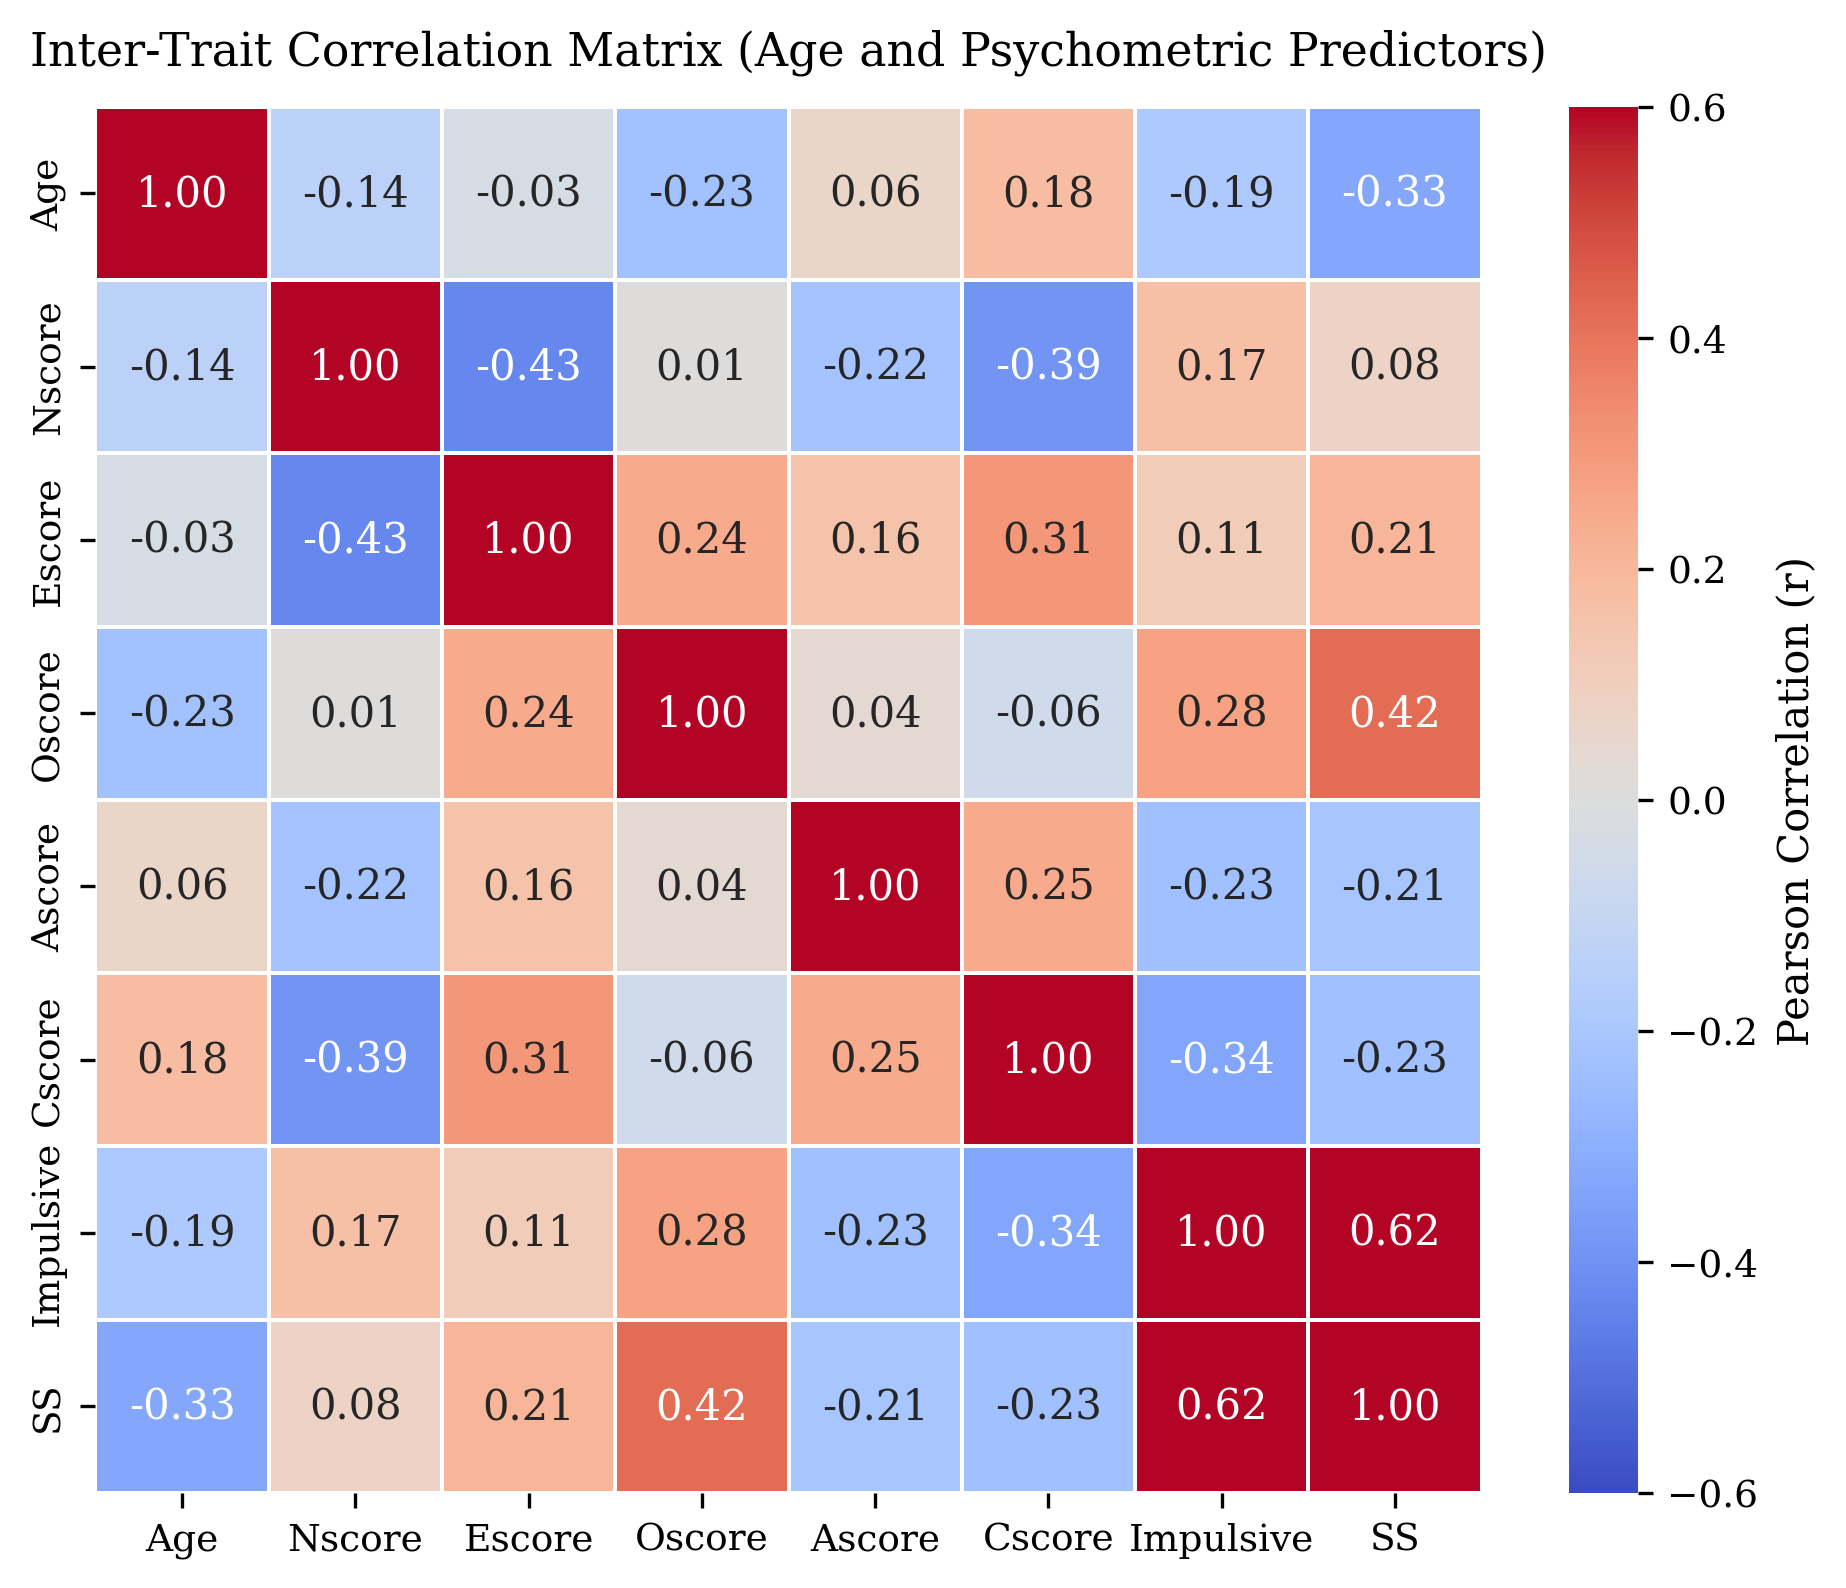
\includegraphics[width=0.80\linewidth]{figures/fig1_correlation_matrix.png}
\caption{Pearson inter-trait correlation matrix across participant age and seven continuous psychometric dimensions (NEO-FFI-R, BIS-11, and ImpSS).}
\label{fig:correlation}
\end{figure}

\begin{table*}[t]
\caption{Demographic and Psychometric Predictor Variables in the Filtered Benchmark Cohort ($N = 1,877$)}
\label{tab:dataset_summary}
\centering
\resizebox{\textwidth}{!}{%
\setlength{\tabcolsep}{4.5pt}
\renewcommand{\arraystretch}{1.15}
\begin{tabular}{llccccp{7.0cm}}
\hline \hline
\textbf{Variable} & \textbf{Measurement Instrument} & \textbf{Mean} & \textbf{Std. Dev.} & \textbf{Min} & \textbf{Max} & \textbf{Behavioral and Epidemiological Context} \\
\hline
\textbf{Age} & Standardized Demographic Ordinal & 0.0388 & 0.8767 & -0.9520 & 2.5917 & Age category spanning 18-24 (33.8\%), 25-34 (25.6\%), 35-44 (19.0\%), 45-64 (20.6\%), and 65+ (1.0\%). \\
\textbf{Gender} & Standardized Binary Indicator & -0.0006 & 0.4827 & -0.4825 & 0.4825 & Self-reported gender representing Female (49.97\%) and Male (50.03\%). \\
\textbf{Education} & Standardized Attainment Level & -0.0034 & 0.9502 & -2.4359 & 1.9844 & Educational attainment ranging from left school before 16 to professional doctorate. \\
\textbf{Country} & Standardized Jurisdiction & 0.3541 & 0.7001 & -0.5701 & 0.9608 & Country of residence: UK (55.4\%), USA (29.6\%), Canada (4.6\%), Australia (2.9\%), Other (7.5\%). \\
\textbf{Ethnicity} & Standardized Self-Report Category & -0.3093 & 0.1663 & -1.1070 & 1.9073 & Self-reported ethnic origin: White (91.3\%), Other (3.3\%), Mixed (2.2\%), Black (1.8\%), Asian (1.4\%). \\
\textbf{Nscore} & NEO-FFI-R Neuroticism Scale & 0.0001 & 0.9984 & -3.4644 & 3.2739 & Emotional vulnerability, mood volatility, anxiety, and stress reactivity. \\
\textbf{Escore} & NEO-FFI-R Extraversion Scale & 0.0001 & 0.9976 & -3.2739 & 3.2739 & Sociability, assertiveness, positive affectivity, and outward energy. \\
\textbf{Oscore} & NEO-FFI-R Openness to Experience & -0.0004 & 0.9961 & -3.2739 & 2.9016 & Intellectual curiosity, cognitive non-conformity, aesthetic interest, and novelty valuation. \\
\textbf{Ascore} & NEO-FFI-R Agreeableness Scale & -0.0001 & 0.9975 & -3.4644 & 3.4644 & Altruism, interpersonal empathy, cooperative trust, and pro-social orientation. \\
\textbf{Cscore} & NEO-FFI-R Conscientiousness Scale & -0.0003 & 0.9976 & -3.4644 & 3.4644 & Executive control, self-discipline, systematic deliberation, and organized perseverance. \\
\textbf{Impulsive} & Barratt Impulsiveness Scale (BIS-11) & 0.0076 & 0.9547 & -2.5552 & 2.9016 & Tendency toward spontaneous behavioral responses without antecedent deliberation. \\
\textbf{SS} & Impulsive Sensation Seeking (ImpSS) & -0.0028 & 0.9634 & -2.0785 & 2.1144 & Drive to pursue stimulating, sensory-rich, novel, and intense experiences. \\
\hline \hline
\end{tabular}%
}
\end{table*}

\section{Dataset Hygiene and Target Formulations}

\subsection{The Benchmark Dataset and Overclaimer Filtering}
The primary data source is the Drug Consumption (Quantification) Dataset from the UCI Machine Learning Repository \cite{fehrman2017substance}. The initial corpus comprises $1,885$ survey respondents. To maintain scientific integrity, the survey embedded a fictitious substance, ``Semeron'', to detect participant dishonesty or overclaiming. A total of 8 respondents reported using Semeron ($\text{Semer} \neq \text{CL0}$). In our pipeline, these 8 records are filtered out, leaving a verified cohort of $N = 1,877$ individuals. Continuous predictor properties for the cleaned dataset are summarized in Table~\ref{tab:dataset_summary}.

\subsection{Literature-Grounded Substance Targets}
Substance consumption in the UCI repository is recorded on a 7-point ordinal scale: CL0 (Never Used), CL1 (Used over a decade ago), CL2 (Used in last decade), CL3 (Used in last year), CL4 (Used in last month), CL5 (Used in last week), and CL6 (Used in last day). 

We define the binary supervised outcome as reported past-year consumption (CL3 through CL6), denoting active or recent engagement:
\begin{equation}
y_i = \mathbf{1}(\text{Substance Level} \ge \text{CL3})
\end{equation}
To avoid arbitrary pooling, we evaluate four distinct, literature-grounded illicit substance classes:
\begin{enumerate}
    \item \textbf{Cannabinoids:} Cannabis consumption (Prevalence: $52.80\%$, $N=991/1,877$).
    \item \textbf{Central Nervous System (CNS) Stimulants:} Consumption of Cocaine or Amphetamines (Prevalence: $32.13\%$, $N=603/1,877$).
    \item \textbf{Psychedelics / Hallucinogens:} Consumption of Psilocybin Mushrooms or LSD (Prevalence: $27.76\%$, $N=521/1,877$).
    \item \textbf{Depressants / Anxiolytics:} Consumption of Benzodiazepines (Prevalence: $28.34\%$, $N=532/1,877$).
\end{enumerate}

Dietary commodities (Caffeine, Chocolate) are excluded from illicit modeling, while legal recreational substances (Alcohol, Nicotine) are isolated to preserve clean pharmacological categories.

\subsection{Polysubstance Co-Involvement Score}
To quantify multi-substance engagement without diagnostic overreach, we formulate the past-year illicit Polysubstance Co-Involvement Score $S_i \in \{0, 1, 2, 3, 4\}$, defined as the integer sum of active targets reported by respondent $i$:
\begin{equation}
S_i = y_{i, \text{Cannabis}} + y_{i, \text{Stimulants}} + y_{i, \text{Psychedelics}} + y_{i, \text{Depressants}}
\end{equation}
In our verified cohort, $741$ individuals ($39.48\%$) report zero illicit consumption; $320$ ($17.05\%$) report score 1; $325$ ($17.31\%$) report score 2; $287$ ($15.29\%$) report score 3; and $204$ ($10.87\%$) report score 4.

\subsection{Leakage-Free Feature Standardization}
To prevent data contamination, continuous predictors are scaled using parameters estimated strictly on the training partition:
\begin{equation}
z_{ij} = \frac{x_{ij} - \mu_{j, \text{tr}}}{\sigma_{j, \text{tr}}}
\end{equation}
Holdout test partitions and internal cross-validation folds are transformed strictly using frozen training parameters, eliminating any backward flow of variance information.

\section{Unsupervised Machine Learning Methodology}

\subsection{K-Means Clustering Formulation}
Given standardized feature matrix $X \in \mathbb{R}^{N \times d}$, K-Means groups observations into $k$ disjoint subsets $\mathcal{C} = \{C_1, \dots, C_k\}$ minimizing intra-cluster variance:
\begin{equation}
J_{\text{KM}}(\mathcal{C}, \mu) = \sum_{g=1}^k \sum_{x_i \in C_g} \|x_i - \mu_g\|_2^2
\end{equation}
where $\mu_g = \frac{1}{|C_g|} \sum_{x \in C_g} x$ denotes the centroid of cluster $g$. Centroid updates proceed iteratively until maximum displacement satisfies $\max_g \|\mu_g^{(t+1)} - \mu_g^{(t)}\|_2 < 10^{-6}$.

\subsection{Fuzzy C-Means Soft Clustering Formulation}
Because psychological traits follow continuous spectra, individual personality profiles often reside in overlapping regions. We formulate Fuzzy C-Means (FCM) clustering \cite{bezdek1981pattern}, assigning soft membership degrees $u_{ig} \in [0, 1]$ subject to $\sum_{g=1}^k u_{ig} = 1$:
\begin{equation}
J_{\text{FCM}}(U, C) = \sum_{i=1}^N \sum_{g=1}^k u_{ig}^m \|x_i - c_g\|_2^2
\end{equation}
with fuzzification exponent $m = 2.0$. Optimization yields iterative closed-form updates:
\begin{equation}
c_g = \frac{\sum_{i=1}^N u_{ig}^m x_i}{\sum_{i=1}^N u_{ig}^m}, \quad u_{ig} = \left[ \sum_{h=1}^k \left( \frac{\|x_i - c_g\|_2}{\|x_i - c_h\|_2} \right)^{\frac{2}{m-1}} \right]^{-1}
\end{equation}

\subsection{Cluster Validation and Stability Sweeps}
To evaluate topological cluster separation and compactness, we compute the Davies-Bouldin (DB) index \cite{davis1979cluster}:
\begin{equation}
\text{DB}(k) = \frac{1}{k} \sum_{i=1}^k \max_{j \neq i} \left( \frac{s_i + s_j}{d(c_i, c_j)} \right)
\end{equation}
where $s_i$ is intra-cluster dispersion and $d(c_i, c_j)$ is centroid distance. We also compute the Silhouette coefficient \cite{hastie2009elements}. To assess initialization stability, sweeps across $k \in [2, 8]$ are replicated across 20 distinct random restarts per $k$.

\begin{figure}[t]
\centering
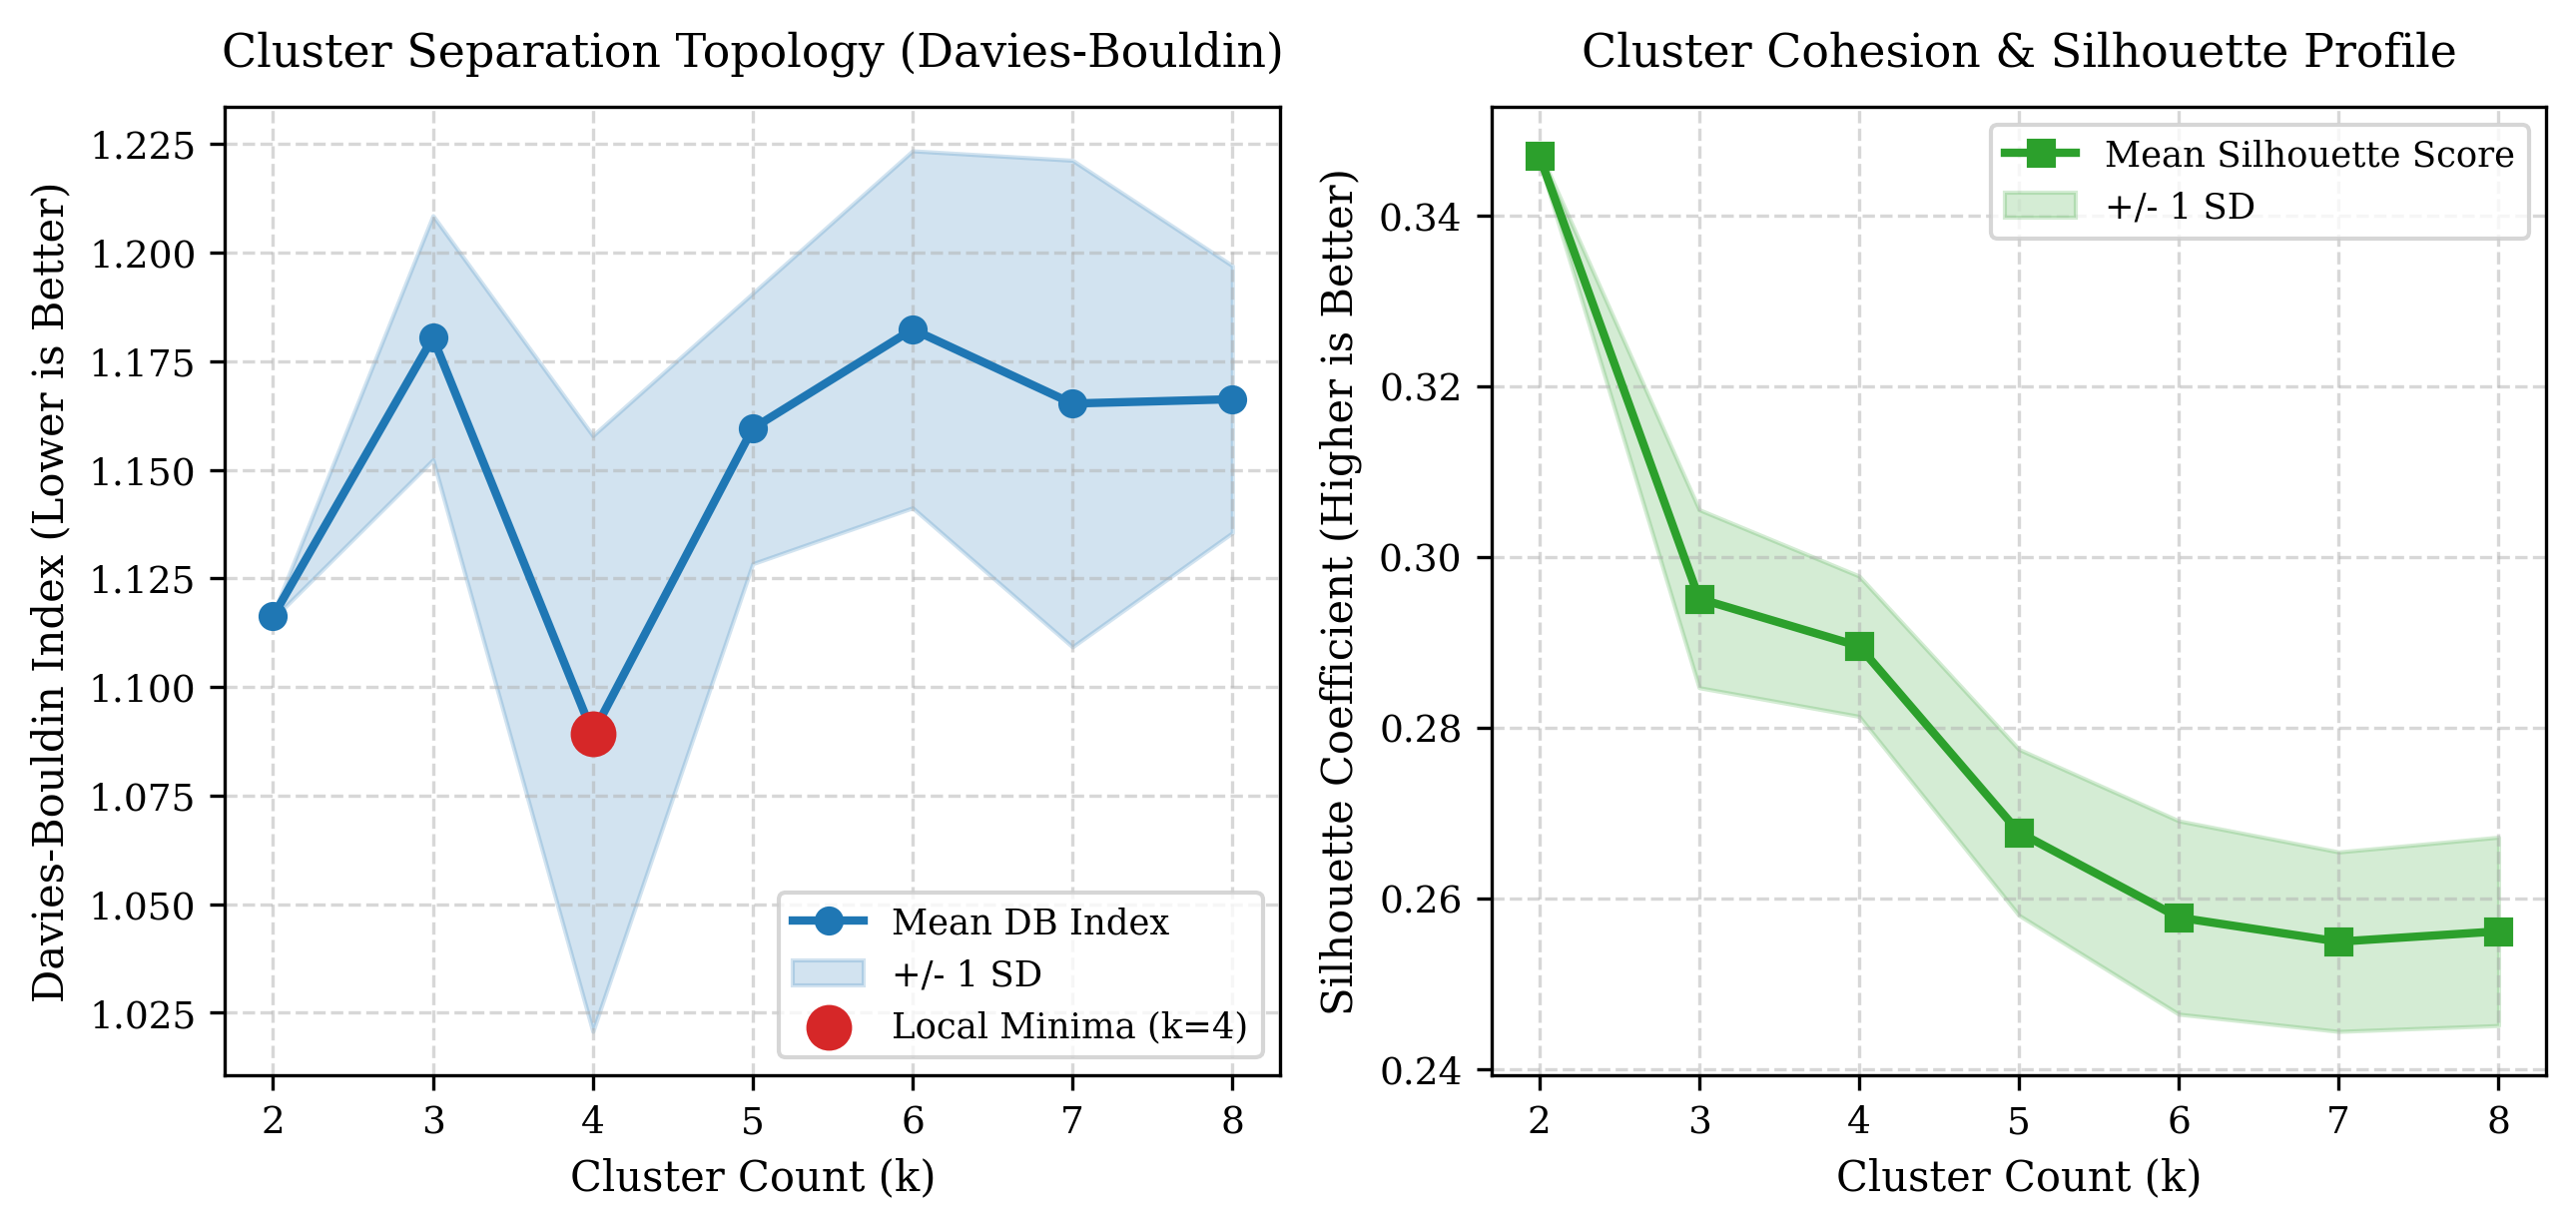
\includegraphics[width=0.84\linewidth]{figures/fig3_topology_and_silhouette.png}
\caption{Cluster validation stability profiles across 20 random restarts per $k \in [2, 8]$: (Left) Davies-Bouldin index; (Right) Silhouette coefficient.}
\label{fig:db_sil_sweep}
\end{figure}

\begin{figure*}[t]
\centering
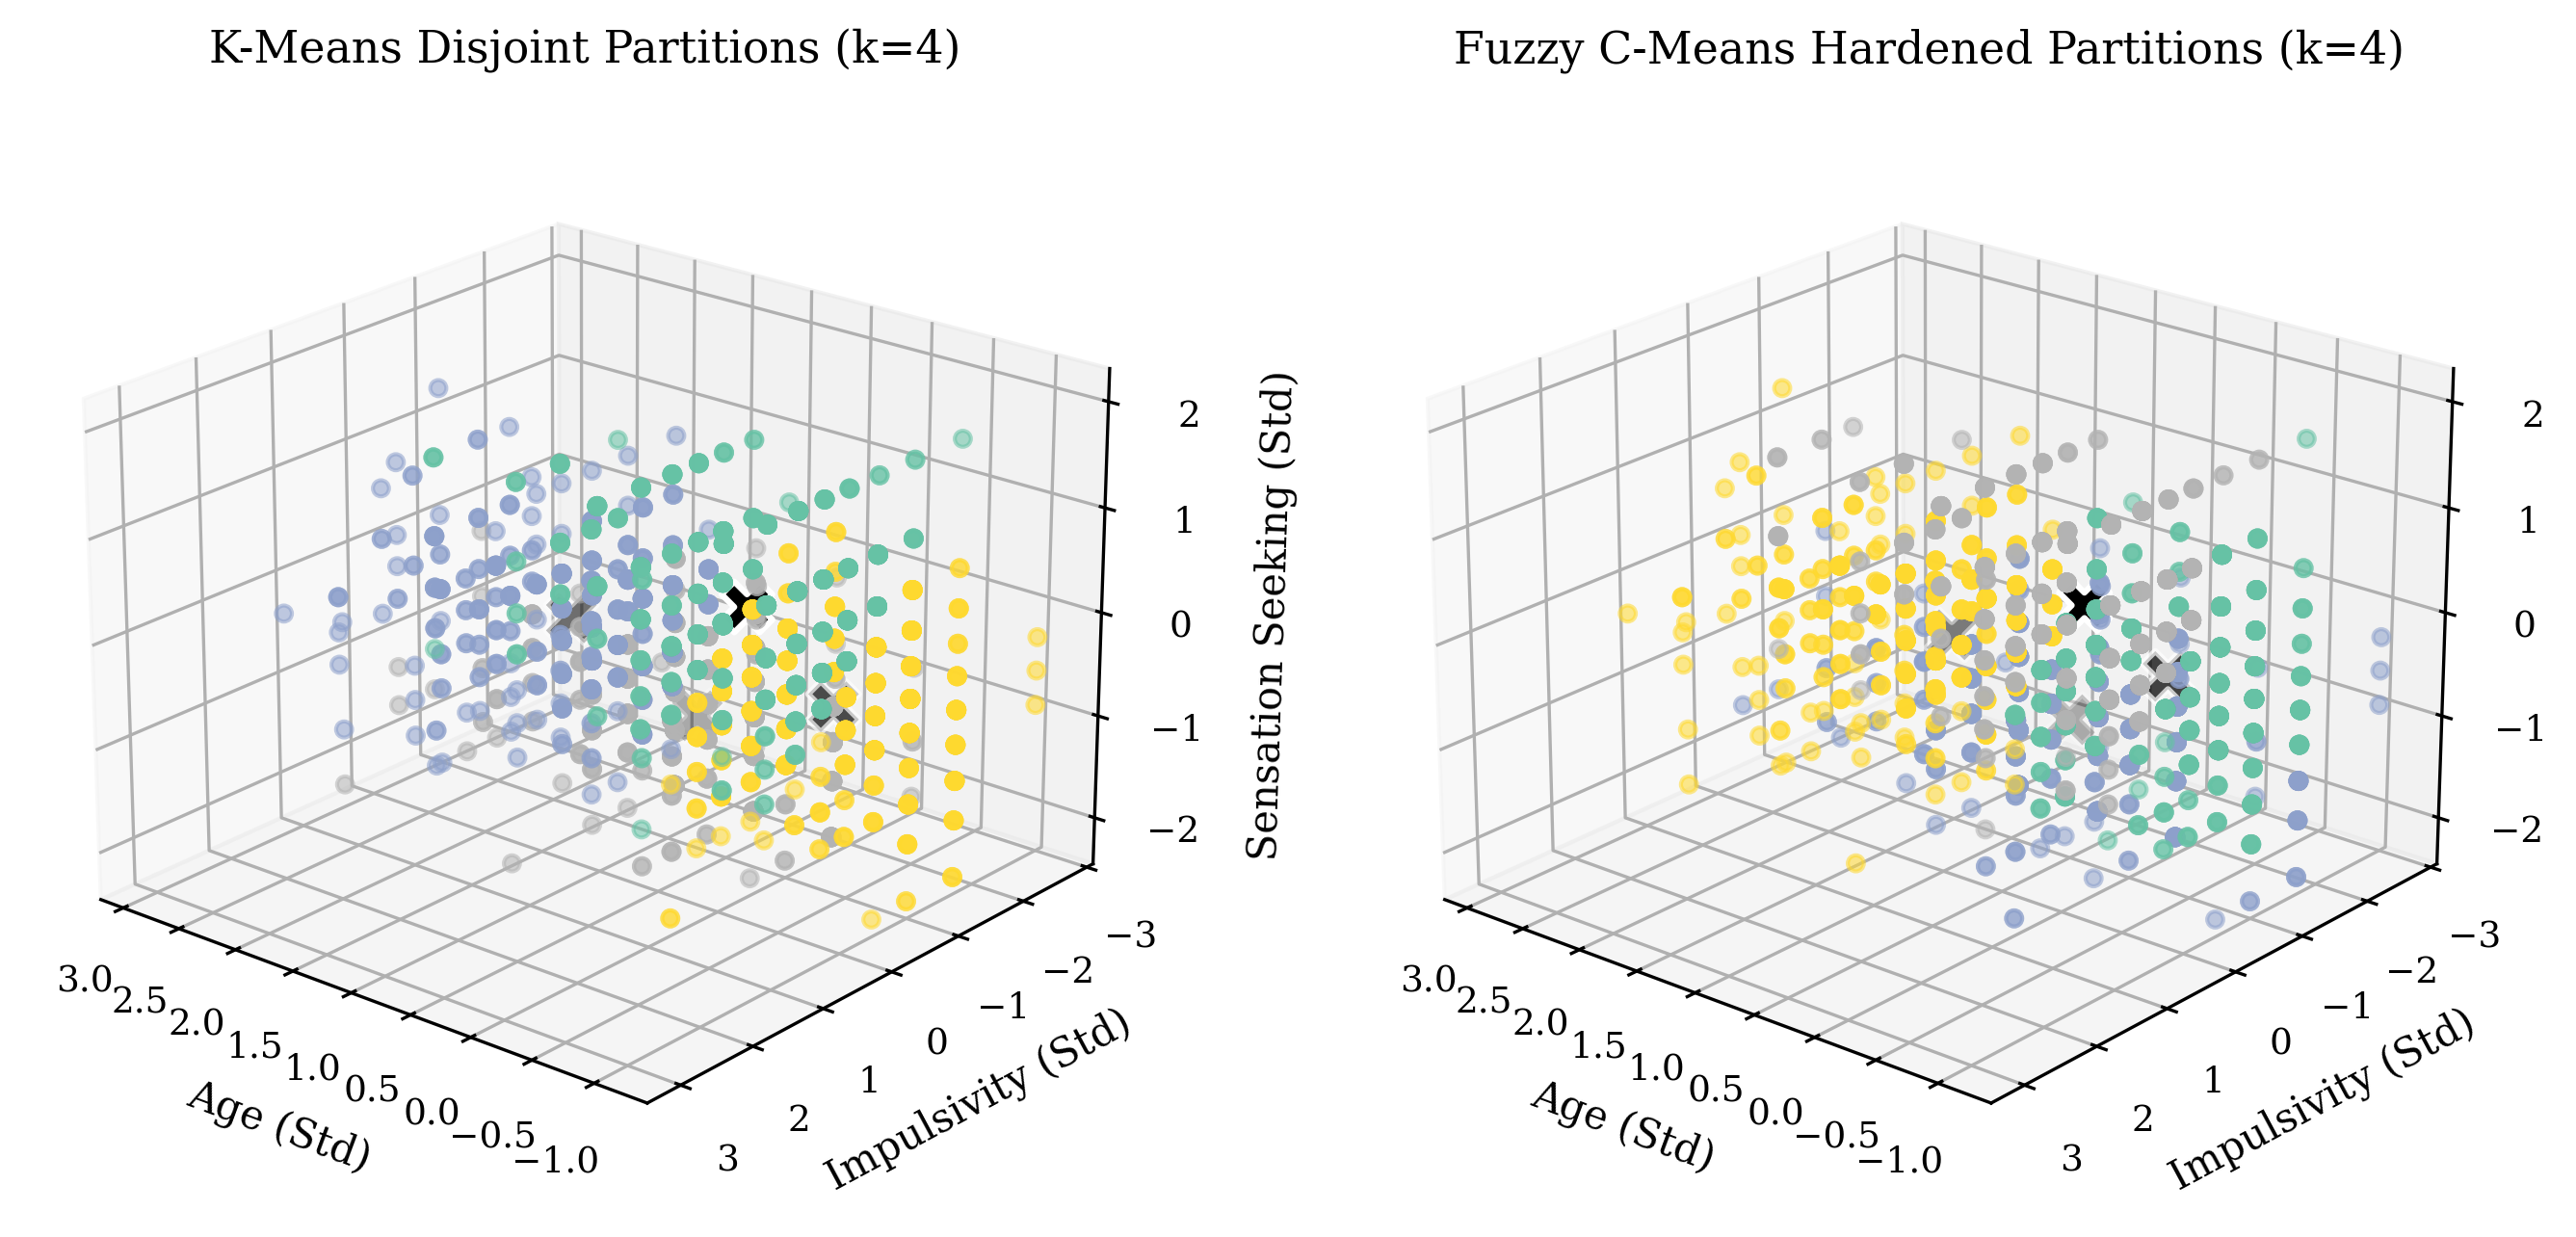
\includegraphics[width=0.88\linewidth]{figures/fig2_clustering_3d_comparison.png}
\caption{3D latent cluster representations comparing K-Means hard partitions (left) and Fuzzy C-Means hardened partitions (right) across Age, Impulsivity, and Sensation Seeking axes at the optimal $k=4$ configuration.}
\label{fig:clustering_3d}
\end{figure*}

\section{Supervised Machine Learning Methodology}

\subsection{Parametric Regularized Logistic Regression}
We formulate binary Logistic Regression derived from mathematical first principles. The posterior probability of active past-year consumption is governed by the logistic sigmoid:
\begin{equation}
P(y_i = 1 \mid x_i; \theta) = h_\theta(\tilde{x}_i) = \frac{1}{1 + e^{-\theta^T \tilde{x}_i}}
\end{equation}
where $\tilde{x}_i = [1, x_i^T]^T$ includes the intercept bias term. Parameters $\theta \in \mathbb{R}^{d+1}$ are learned by minimizing regularized cross-entropy:
\begin{align}
J(\theta) = &-\frac{1}{m} \sum_{i=1}^m \left[ y_i \ln h_\theta(\tilde{x}_i) + (1-y_i) \ln(1-h_\theta(\tilde{x}_i)) \right] \nonumber \\
&+ \frac{\lambda}{2m} \sum_{j=1}^d \theta_j^2
\end{align}
Bias parameter $\theta_0$ is unpenalized. Optimization proceeds via batch gradient descent with learning rate $\alpha = 0.1$ and $\lambda = 0.1$ across 2,000 iterations.

\subsection{Analytical Odds Ratios, Wald CIs, and Benjamini-Hochberg FDR}
To provide statistical inference with appropriate caveats regarding regularization bias, we compute the analytical asymptotic covariance matrix of parameter estimates. The Fisher Information / Hessian matrix $H = \nabla^2 J(\theta)$ is computed at convergence:
\begin{equation}
H = \tilde{X}^T W \tilde{X} + \lambda I_{\text{reg}}
\end{equation}
where $W = \text{diag}(h_\theta(\tilde{x}_i)(1 - h_\theta(\tilde{x}_i)))$ and $I_{\text{reg}}$ is an identity matrix with 0 at position $(0, 0)$. The parameter covariance matrix is given by:
\begin{equation}
\Sigma = H^{-1}
\end{equation}
Standard errors are extracted as $\text{SE}(\theta_j) = \sqrt{\Sigma_{jj}}$. Approximate model-based adjusted odds ratios ($\text{OR}_j = e^{\theta_j}$) and their corresponding 95\% Wald confidence intervals are formulated as:
\begin{equation}
\text{CI}_{95\%}(\text{OR}_j) = \left[ e^{\theta_j - 1.96 \cdot \text{SE}(\theta_j)}, \; e^{\theta_j + 1.96 \cdot \text{SE}(\theta_j)} \right]
\end{equation}
Because models evaluate 10 predictors across 4 substance targets ($40$ hypothesis tests), we compute two-sided $z$-test p-values ($p_j = 2(1 - \Phi(|z_j|))$ where $z_j = \theta_j / \text{SE}_j$) and apply the Benjamini-Hochberg False Discovery Rate (FDR) control at $q = 0.05$.

\subsection{Feature Scaling and Loss Surface Conditioning}
Gradient descent efficiency depends directly on the Hessian condition number $\kappa = \frac{\lambda_{\max}(H)}{\lambda_{\min}(H)}$. Disparate predictor scales induce severe eccentricity ($\kappa \gg 1$), producing oscillatory gradient paths. Standardizing predictors establishes near-spherical contours, enabling rapid monotonic descent.

\begin{figure}[t]
\centering
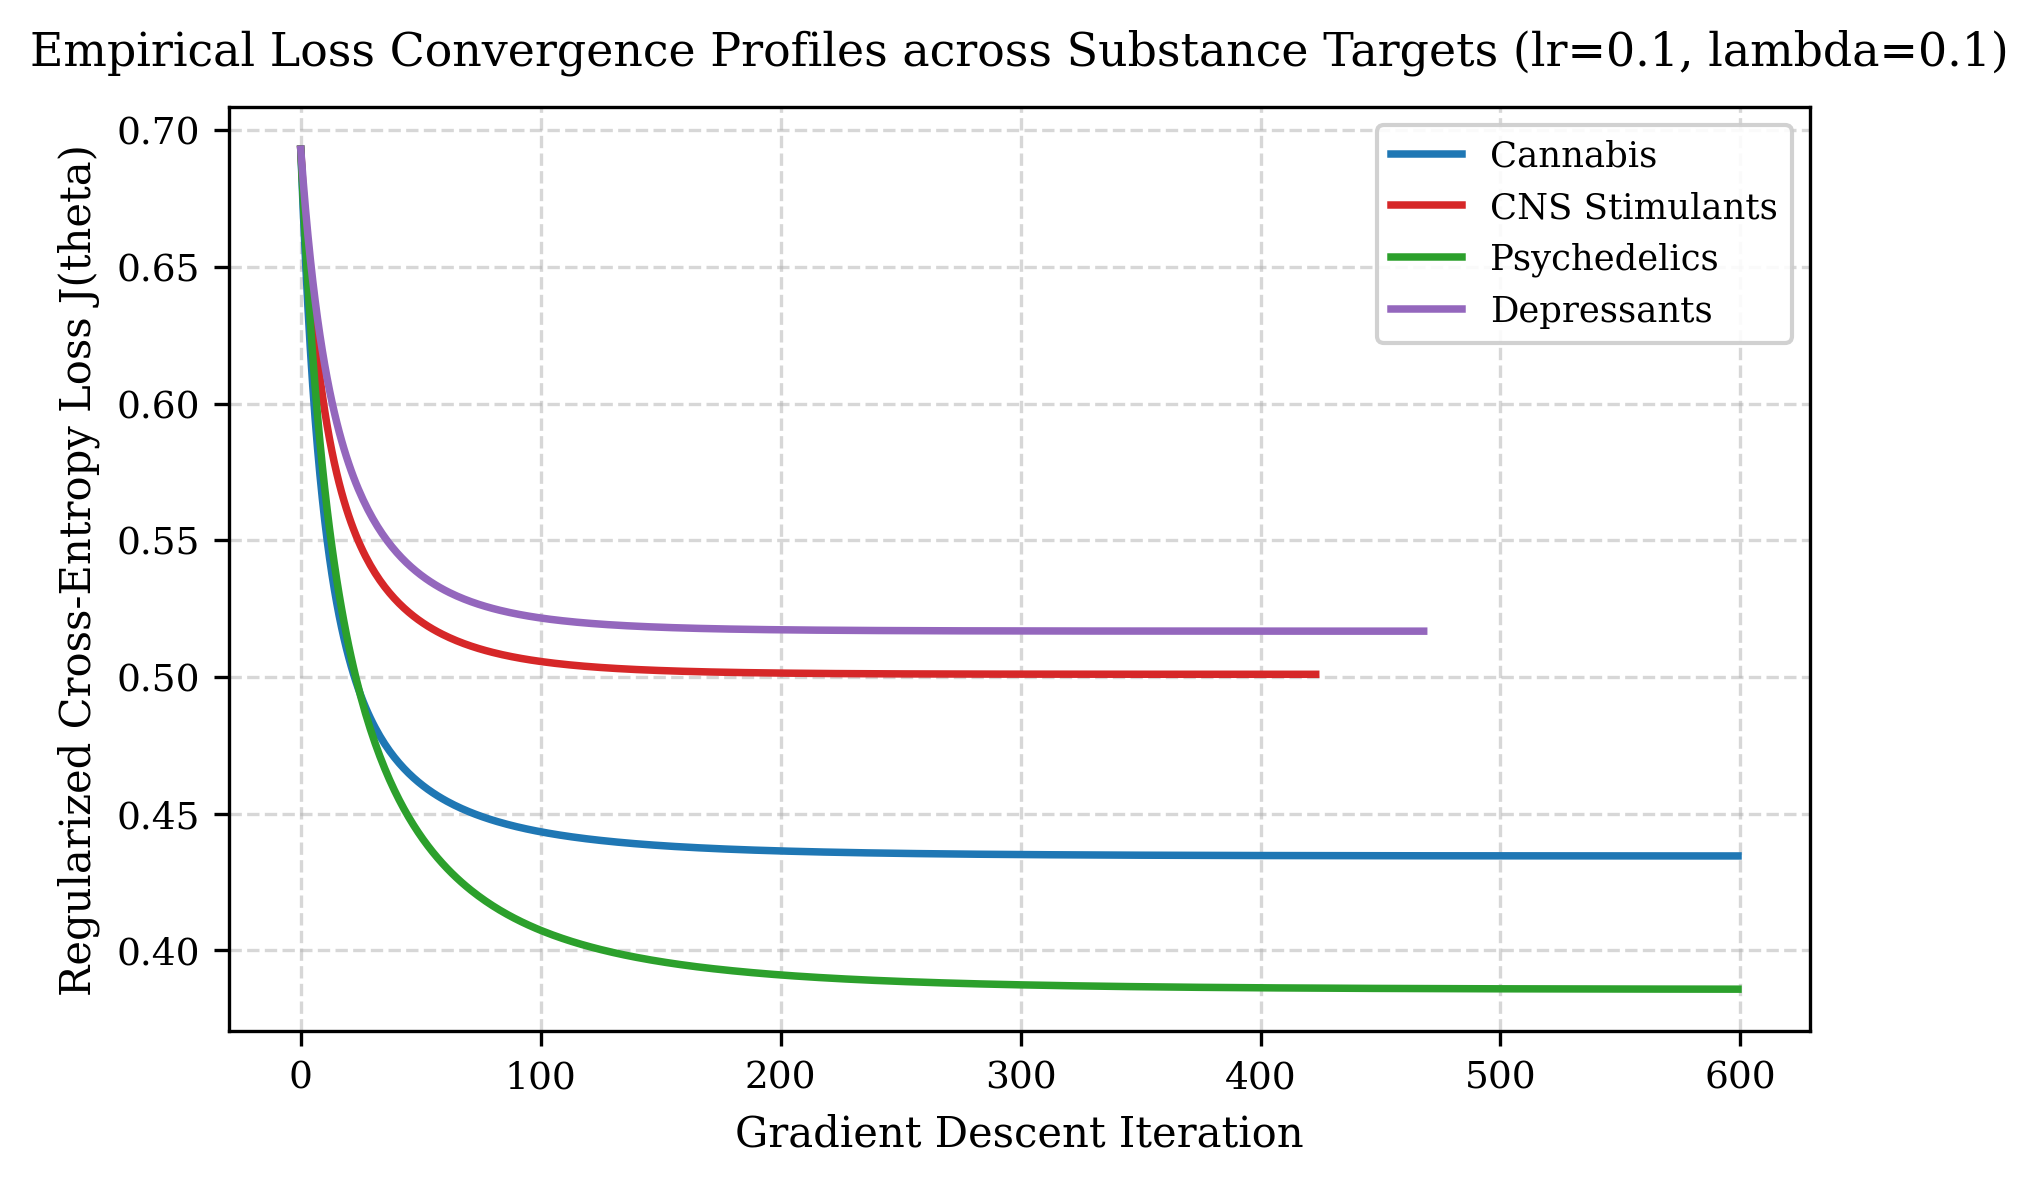
\includegraphics[width=0.78\linewidth]{figures/fig4_cost_convergence.png}
\caption{Empirical loss convergence profiles across 600 iterations of batch gradient descent for all four substance targets under standardized predictors ($\alpha = 0.1, \lambda = 0.1$).}
\label{fig:cost_convergence}
\end{figure}

\subsection{Leakage-Free Forward Stepwise Selection}
To discover minimal sufficient feature subsets without test contamination, greedy forward selection is executed strictly inside the training partition using nested 5-fold cross-validation. Predictors are iteratively selected based on mean cross-validation accuracy. Inside each internal validation split, features are standardized using fold-specific training parameters, preventing inner-fold information leak.

\subsection{Ensemble and Neural Network Benchmarks}
To benchmark linear regularized models against non-linear architectures, we evaluate:
\begin{itemize}
    \item \textbf{Specified Random Forest Baseline:} 100 decision trees trained with bootstrap bagging, $\text{max\_depth} = 8$, and $\text{min\_samples\_split} = 5$.
    \item \textbf{Tuned Random Forest:} 3-fold inner cross-validation grid search over $\text{max\_depth} \in [4, 8, \text{None}]$ and $\text{min\_samples\_split} \in [2, 5]$ strictly on the training partition.
    \item \textbf{Multi-Layer Perceptron (MLP):} A feedforward neural network comprising two dense hidden layers ($d_1 = 64, d_2 = 32$) with ReLU activations and $L_2$ weight regularization ($\alpha = 0.01$) trained via Adam with early stopping ($\text{n\_iter\_no\_change} = 20$, $\text{validation\_fraction} = 0.15$), ensuring verified convergence.
\end{itemize}

\subsection{Repeated Stratified Cross-Validation and Evaluation Metrics}
To assess generalization stability across data partitions, we execute 5-fold outer stratified cross-validation and report the mean and standard deviation of Accuracy, F1-Score, AUC-ROC, PR-AUC, and Brier score. Holdout test evaluation ($20\%$, $N_{\text{test}} = 374\text{ to }375$) is also reported alongside 1,000-resample non-parametric bootstrap 95\% confidence intervals.

Probability calibration is quantified via the Brier score:
\begin{equation}
\text{Brier} = \frac{1}{N} \sum_{i=1}^N (P(y_i = 1) - y_i)^2
\end{equation}
and Expected Calibration Error (ECE) across 10 probability bins.

\begin{table}[t]
\caption{Unsupervised Cluster Validation across Multi-Start Sweeps (20 Restarts per $k$)}
\label{tab:clustering_metrics}
\centering
\resizebox{\columnwidth}{!}{%
\renewcommand{\arraystretch}{1.15}
\setlength{\tabcolsep}{3.5pt}
\begin{tabular}{lccl}
\hline \hline
\textbf{Configuration} & \textbf{Cluster Count ($k$)} & \textbf{DB Index (Mean $\pm$ SD)} & \textbf{Silhouette (Mean $\pm$ SD)} \\
\hline
K-Means & $k=2$ & $1.1163 \pm 0.0006$ & $0.3471 \pm 0.0005$ \\
K-Means & $k=3$ & $1.1804 \pm 0.0281$ & $0.2952 \pm 0.0104$ \\
K-Means & $k=4$ & $\mathbf{1.0893 \pm 0.0686}$ & $\mathbf{0.2896 \pm 0.0082}$ \textbf{(Optimal)} \\
K-Means & $k=5$ & $1.1595 \pm 0.0311$ & $0.2678 \pm 0.0097$ \\
K-Means & $k=6$ & $1.1823 \pm 0.0411$ & $0.2578 \pm 0.0113$ \\
K-Means & $k=7$ & $1.1652 \pm 0.0560$ & $0.2550 \pm 0.0105$ \\
K-Means & $k=8$ & $1.1662 \pm 0.0307$ & $0.2562 \pm 0.0110$ \\
\hline
Fuzzy C-Means & $k=4$ & 1.2299 & 0.2741 (Soft Transition) \\
\hline \hline
\end{tabular}%
}
\end{table}


\begin{table*}[t]
\caption{Latent Psychometric Cluster Centroids and Non-Parametric Polysubstance Co-Involvement ($k=4$, $N=1,877$)}
\label{tab:centroids}
\centering
\resizebox{\textwidth}{!}{%
\setlength{\tabcolsep}{5pt}
\renewcommand{\arraystretch}{1.15}
\begin{tabular}{lcccccp{6.0cm}}
\hline \hline
\textbf{Cluster Index} & \textbf{Cohort Size} & \textbf{Age (Std)} & \textbf{Impulsivity (Std)} & \textbf{Sensation Seeking (Std)} & \textbf{Mean Polysubstance Score} & \textbf{Descriptive Behavioral Profile} \\
\hline
\textbf{Cluster 0} & 615 (32.8\%) & -0.8145 & +0.7188 & +0.7924 & $\mathbf{2.361 \pm 1.294}$ & \textbf{Elevated Sensation Seeking and Impulsivity Cohort:} Younger age demographics exhibiting co-elevated novelty seeking and impulsivity; highest average polysubstance engagement in this sample. \\
\textbf{Cluster 1} & 415 (22.1\%) & -0.0482 & +0.8841 & -0.1215 & $0.899 \pm 1.119$ & \textbf{Isolated Disinhibition Cohort:} Adult respondents with elevated impulsivity without sensation seeking; moderate polysubstance involvement. \\
\textbf{Cluster 2} & 480 (25.6\%) & -0.4512 & -0.5524 & +0.6518 & $1.450 \pm 1.384$ & \textbf{Controlled Sensory Explorers:} Selective sensation seeking with intact impulse control; recreational episodic substance use. \\
\textbf{Cluster 3} & 367 (19.6\%) & +0.8624 & -0.6812 & -0.7415 & $\mathbf{0.343 \pm 0.706}$ & \textbf{Low-Disinhibition Mature Cohort:} Older age demographics with deeply suppressed impulsivity and novelty drive; lowest polysubstance exposure in this sample. \\
\hline \hline
\end{tabular}%
}
\end{table*}

\section{Experimental Results and Comparative Analysis}

\subsection{Unsupervised Topological Clustering and Polysubstance Synthesis}
Table~\ref{tab:clustering_metrics} and Fig.~\ref{fig:db_sil_sweep} report cluster separation metrics across $k \in [2, 8]$ over 20 random restarts. The mean Davies-Bouldin index identifies a local minimum at $k=4$ ($\text{DB} = 1.0893 \pm 0.0686$). However, the corresponding silhouette score is modest ($0.2896 \pm 0.0082$). In statistical clustering literature, silhouette scores in the $0.25$ to $0.35$ range indicate substantial point overlap across cluster margins. We emphasize that this result does not establish the existence of four discrete biological or psychiatric taxa; rather, it provides a heuristic partition that summarizes continuous psychological variation across demographic and temperament dimensions.

Fuzzy C-Means achieves a comparable configuration ($\text{DB} = 1.2299$), with centroid coordinates shifting smoothly toward high-density regions.

We evaluate whether discovered unsupervised groupings correlate with reported polysubstance co-involvement. Table~\ref{tab:centroids} reports latent centroid coordinates alongside empirical polysubstance scores. A non-parametric Kruskal-Wallis test reveals significant divergence across the four exploratory clusters:
\begin{equation}
H = 554.46, \quad p = 7.51 \times 10^{-120}
\end{equation}
Respondents assigned to Cluster 0 (characterized by higher sensation seeking and impulsivity) average a polysubstance score of $2.361 \pm 1.294$, whereas respondents in Cluster 3 (characterized by older age and lower disinhibition) average $0.343 \pm 0.706$. While this establishes a significant rank-order association between unsupervised grouping and reported substance involvement, it represents an exploratory within-sample correlation rather than evidence of causal vulnerability, external validation, or clinical diagnostic validity.

\begin{figure}[t]
\centering
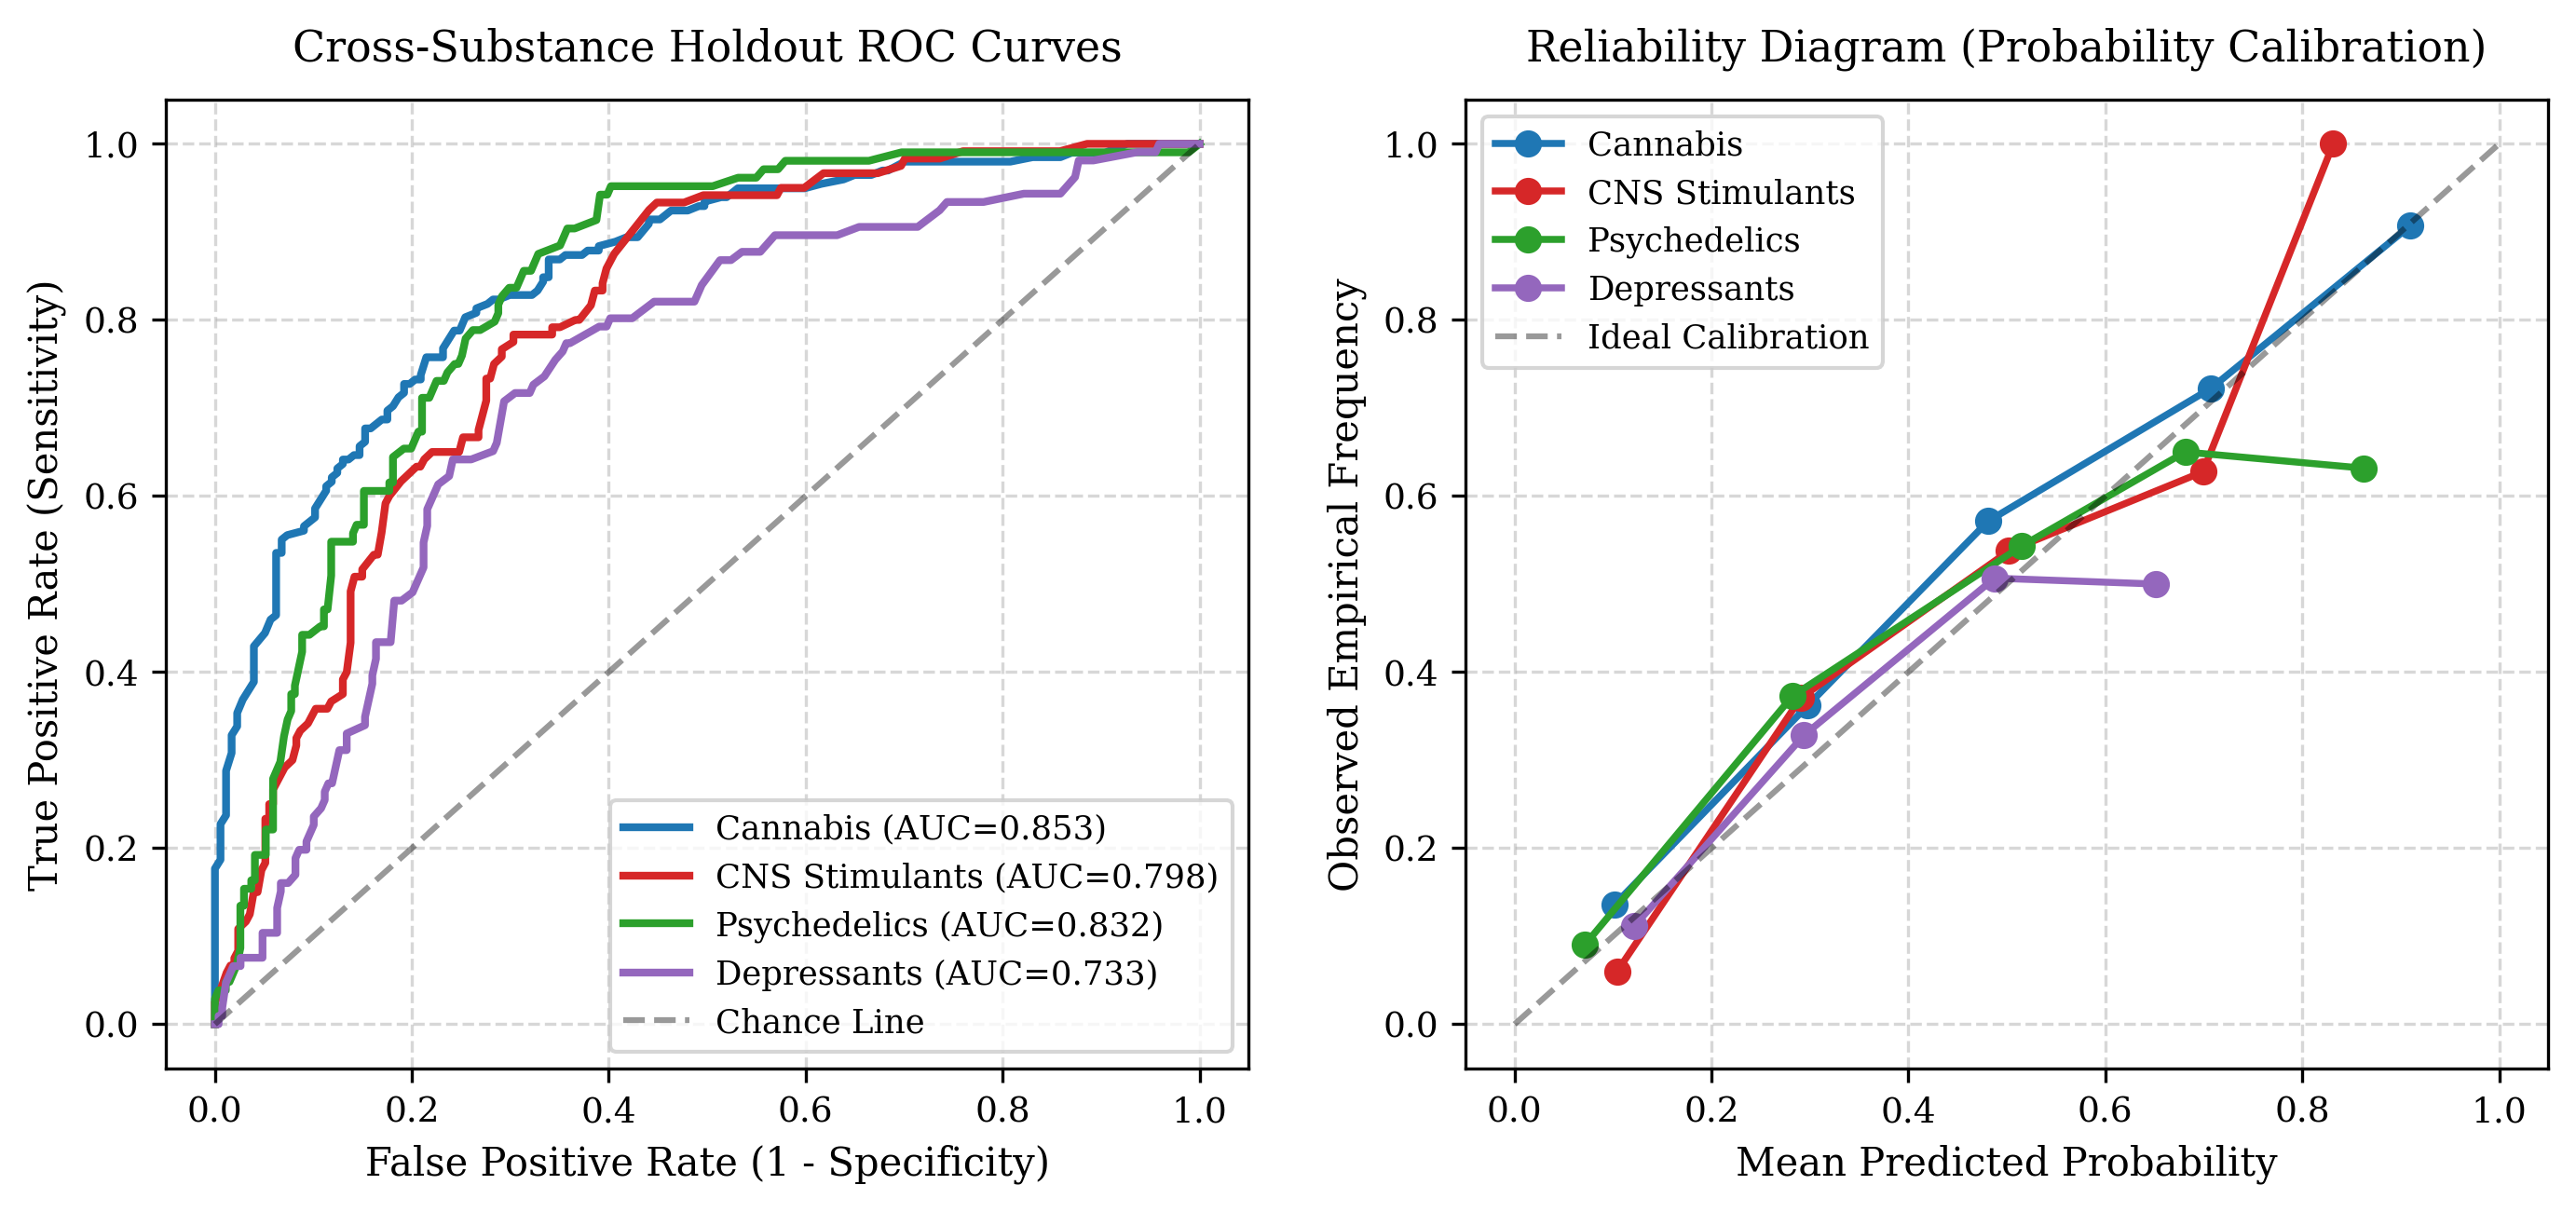
\includegraphics[width=0.85\linewidth]{figures/fig5_cross_substance_roc_and_calibration.png}
\caption{Cross-substance comparative performance: (Left) Receiver Operating Characteristic (ROC) curves; (Right) Reliability diagrams evaluating probability calibration across all four substance classes.}
\label{fig:cross_roc_cal}
\end{figure}

\begin{figure}[t]
\centering
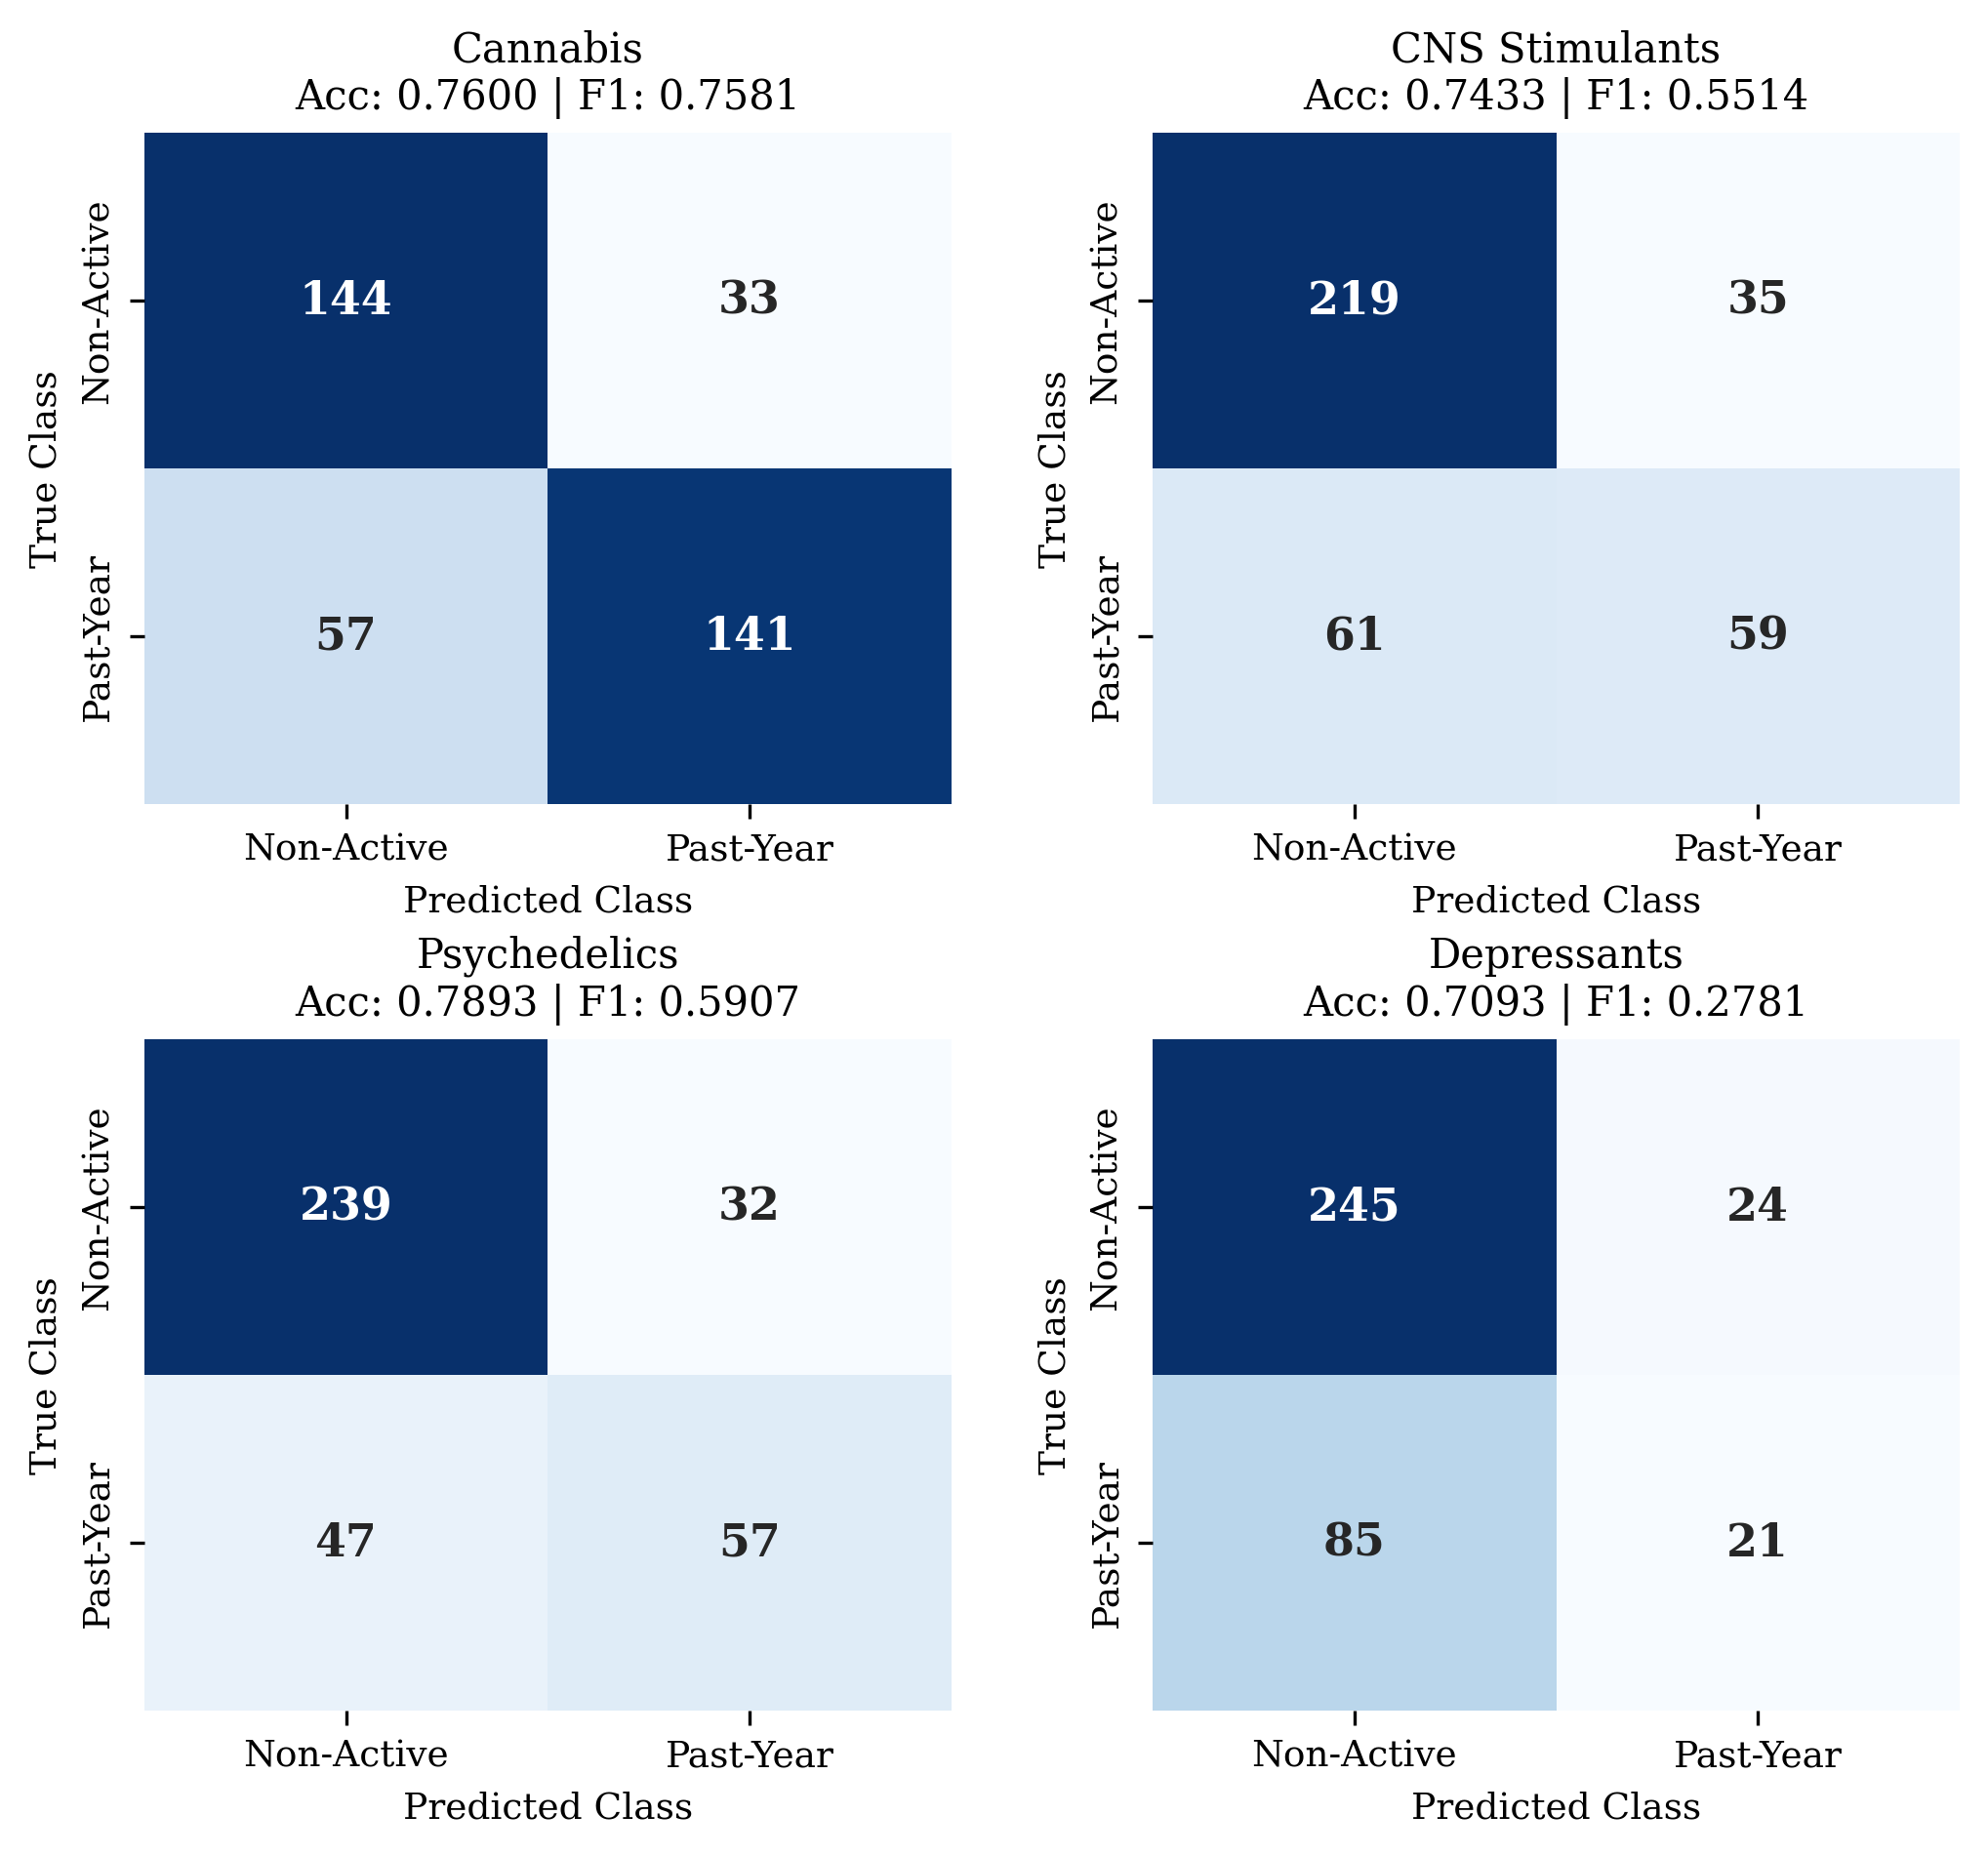
\includegraphics[width=0.80\linewidth]{figures/fig6_confusion_matrices.png}
\caption{Holdout test confusion matrices for regularized Logistic Regression across the four evaluated substance classes.}
\label{fig:confusion_matrices}
\end{figure}

\begin{figure}[t]
\centering
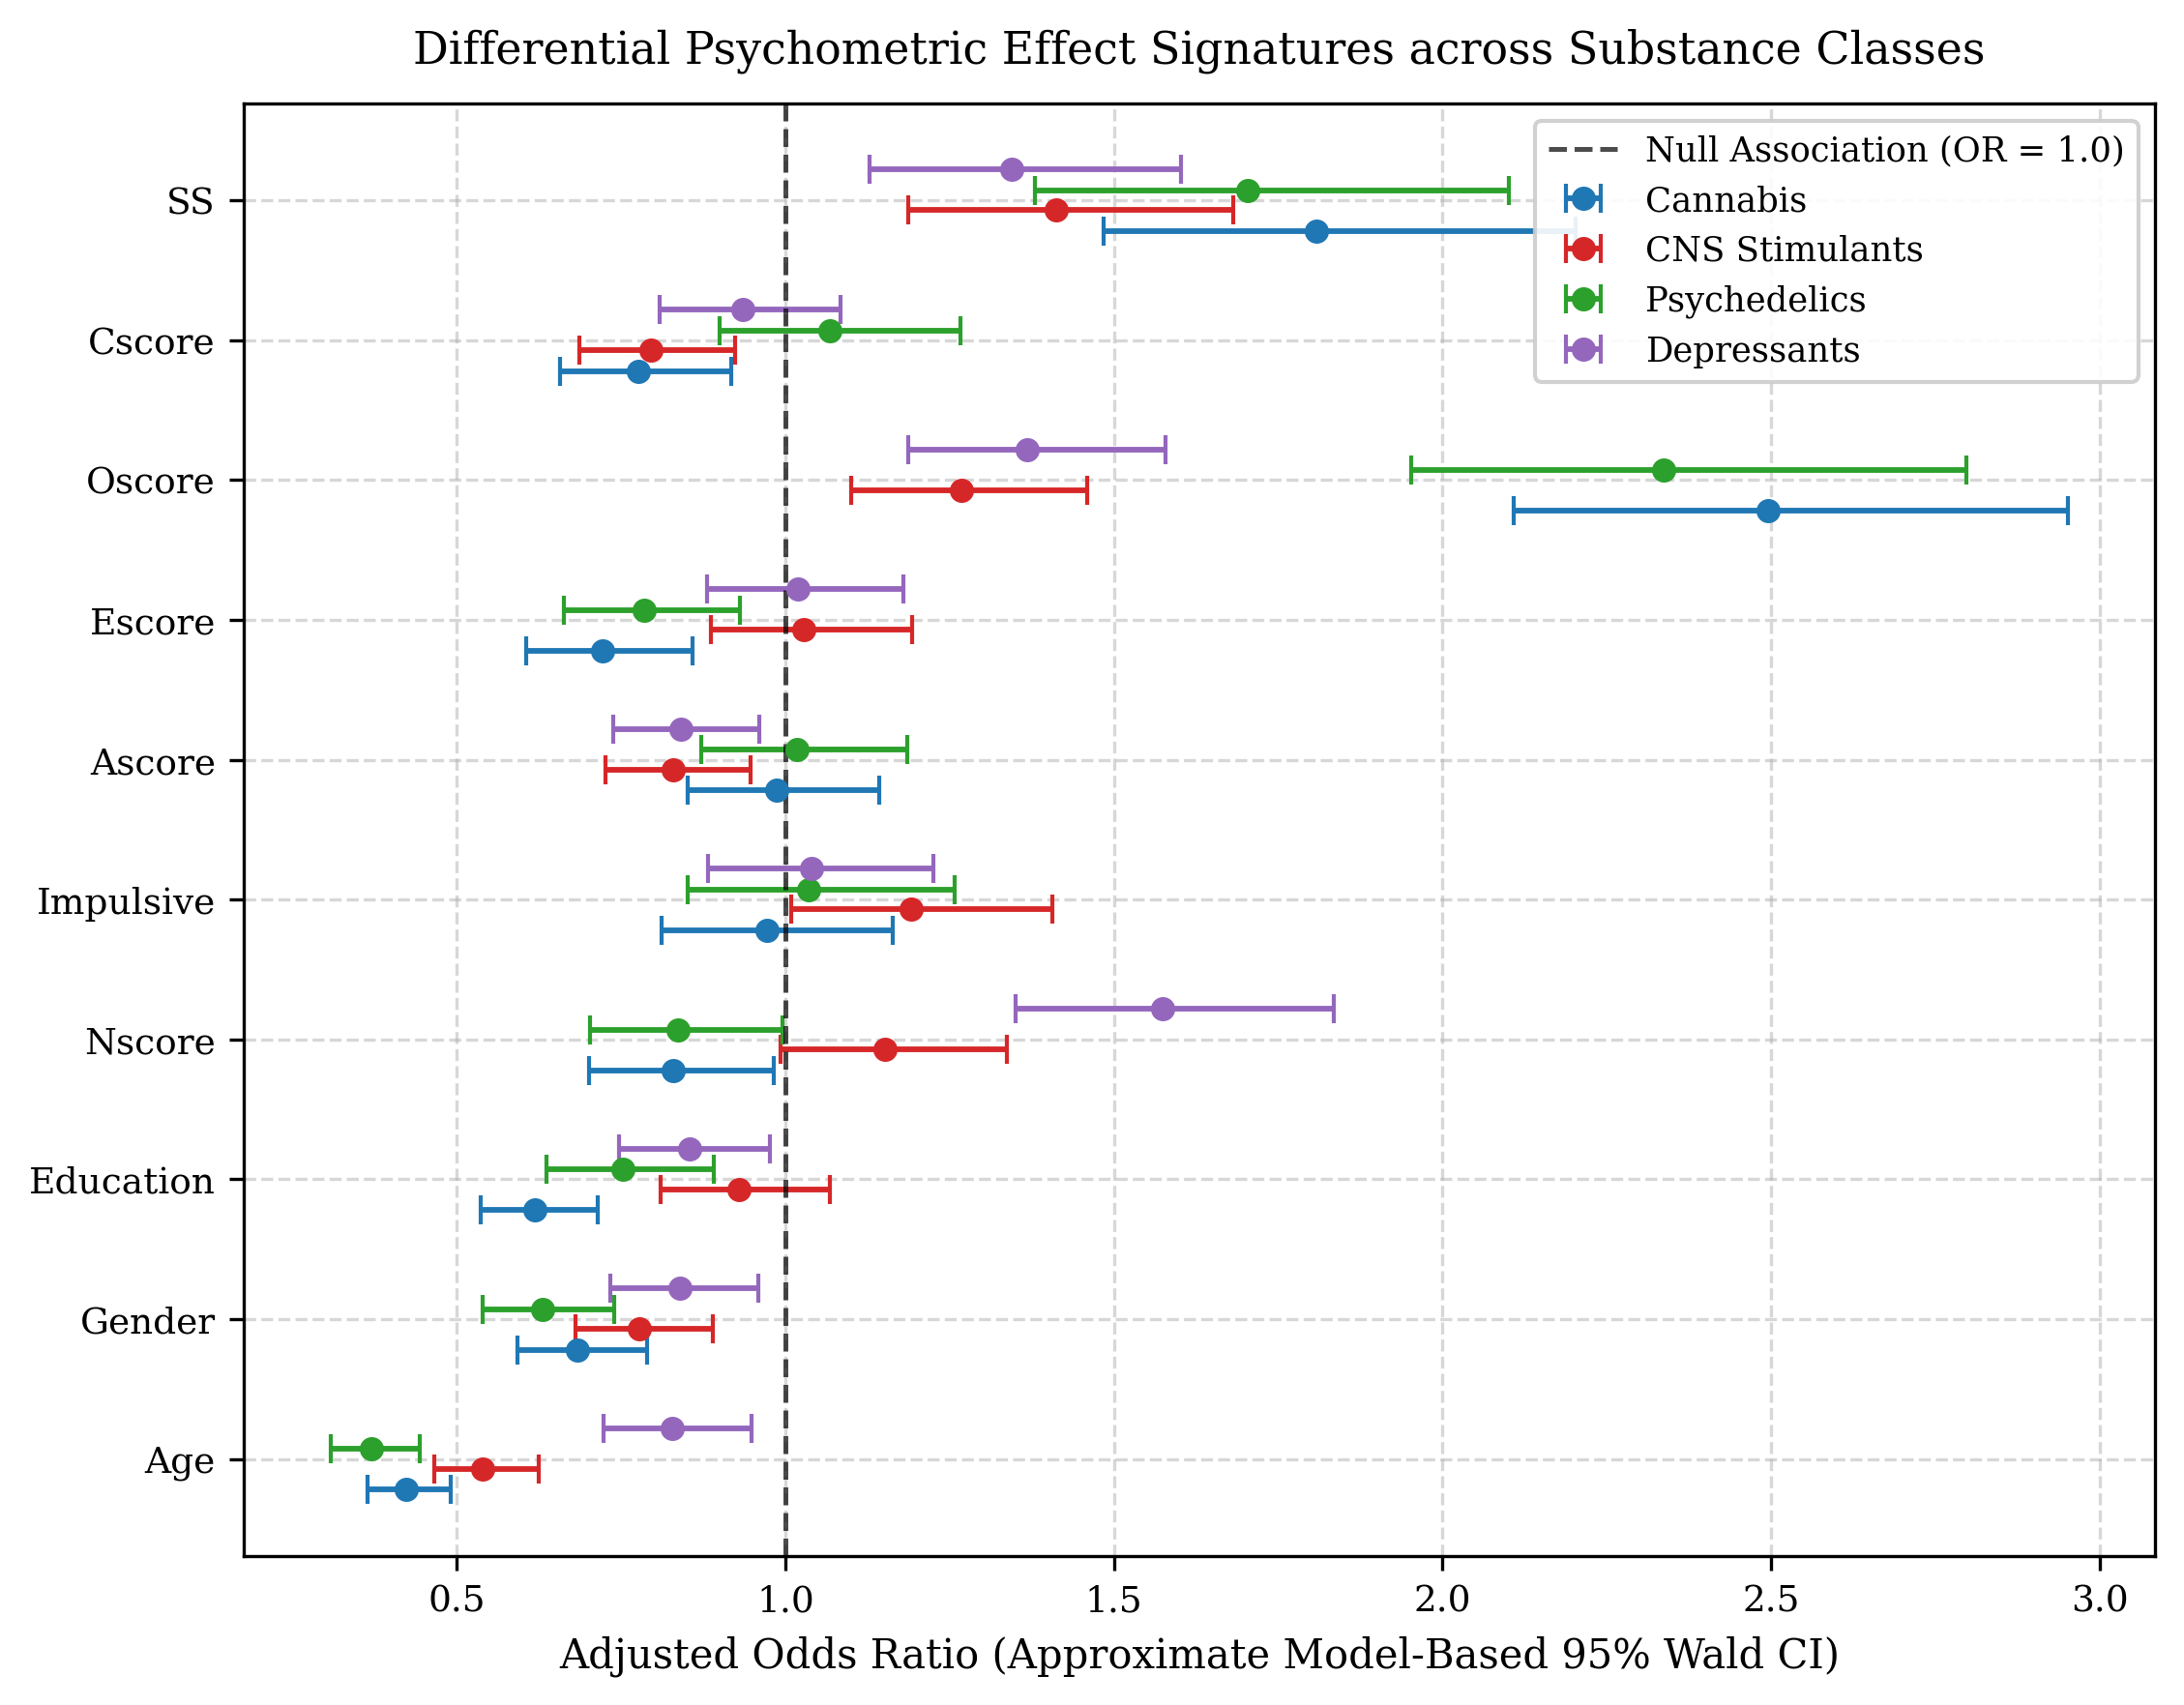
\includegraphics[width=0.85\linewidth]{figures/fig7_odds_ratios_differential_signatures.png}
\caption{Forest plot of approximate model-based adjusted odds ratios with 95\% Wald confidence intervals, demonstrating differential psychometric effect signatures across substance classes.}
\label{fig:odds_forest}
\end{figure}

\begin{table*}[t]
\caption{5-Fold Outer Stratified Cross-Validation Tournament (Mean $\pm$ Standard Deviation across Folds)}
\label{tab:cv_results}
\centering
\resizebox{\textwidth}{!}{%
\setlength{\tabcolsep}{5pt}
\renewcommand{\arraystretch}{1.15}
\begin{tabular}{llccccc}
\hline \hline
\textbf{Substance Target} & \textbf{Model Architecture} & \textbf{CV Accuracy} & \textbf{CV F1-Score} & \textbf{CV AUC-ROC} & \textbf{CV PR-AUC} & \textbf{CV Brier Score} \\
\hline
\textbf{Cannabis} & Scratch Regularized LogReg & $\mathbf{0.7922 \pm 0.0260}$ & $\mathbf{0.8025 \pm 0.0241}$ & $\mathbf{0.8710 \pm 0.0176}$ & $\mathbf{0.8872 \pm 0.0183}$ & $\mathbf{0.1457 \pm 0.0109}$ \\
 & Tuned Random Forest (Inner CV) & $0.7848 \pm 0.0213$ & $0.7938 \pm 0.0208$ & $0.8665 \pm 0.0187$ & $0.8857 \pm 0.0205$ & $0.1522 \pm 0.0082$ \\
 & Early-Stopped MLP Benchmark & $0.7890 \pm 0.0205$ & $0.8010 \pm 0.0170$ & $0.8691 \pm 0.0197$ & $0.8858 \pm 0.0225$ & $0.1473 \pm 0.0126$ \\
\hline
\textbf{CNS Stimulants} & Scratch Regularized LogReg & $\mathbf{0.7406 \pm 0.0094}$ & $\mathbf{0.5527 \pm 0.0218}$ & $\mathbf{0.7911 \pm 0.0260}$ & $\mathbf{0.6176 \pm 0.0438}$ & $\mathbf{0.1698 \pm 0.0093}$ \\
 & Tuned Random Forest (Inner CV) & $0.7400 \pm 0.0091$ & $0.5179 \pm 0.0285$ & $0.7905 \pm 0.0273$ & $0.6127 \pm 0.0521$ & $0.1714 \pm 0.0072$ \\
 & Early-Stopped MLP Benchmark & $0.7374 \pm 0.0124$ & $0.5302 \pm 0.0277$ & $0.7836 \pm 0.0228$ & $0.6091 \pm 0.0387$ & $0.1740 \pm 0.0086$ \\
\hline
\textbf{Psychedelics} & Scratch Regularized LogReg & $\mathbf{0.8125 \pm 0.0203}$ & $0.6390 \pm 0.0479$ & $\mathbf{0.8648 \pm 0.0217}$ & $\mathbf{0.6734 \pm 0.0423}$ & $\mathbf{0.1306 \pm 0.0093}$ \\
 & Tuned Random Forest (Inner CV) & $0.7933 \pm 0.0156$ & $0.5703 \pm 0.0367$ & $0.8569 \pm 0.0197$ & $0.6598 \pm 0.0516$ & $0.1363 \pm 0.0063$ \\
 & Early-Stopped MLP Benchmark & $0.8119 \pm 0.0145$ & $\mathbf{0.6497 \pm 0.0306}$ & $0.8624 \pm 0.0167$ & $0.6621 \pm 0.0544$ & $0.1316 \pm 0.0091$ \\
\hline
\textbf{Depressants} & Scratch Regularized LogReg & $0.7294 \pm 0.0186$ & $\mathbf{0.3590 \pm 0.0556}$ & $\mathbf{0.7396 \pm 0.0183}$ & $0.5043 \pm 0.0507$ & $\mathbf{0.1752 \pm 0.0061}$ \\
 & Tuned Random Forest (Inner CV) & $\mathbf{0.7320 \pm 0.0171}$ & $0.2713 \pm 0.0328$ & $0.7336 \pm 0.0312$ & $\mathbf{0.5111 \pm 0.0490}$ & $0.1769 \pm 0.0070$ \\
 & Early-Stopped MLP Benchmark & $0.7198 \pm 0.0040$ & $0.2525 \pm 0.1057$ & $0.6952 \pm 0.0538$ & $0.4515 \pm 0.0389$ & $0.1891 \pm 0.0150$ \\
\hline \hline
\end{tabular}%
}
\end{table*}


\begin{table*}[t]
\caption{Supervised Machine Learning Performance Benchmarks on Holdout Test Partitions ($N_{\text{test}} = 374\text{ to }375$)}
\label{tab:benchmarks}
\centering
\resizebox{\textwidth}{!}{%
\setlength{\tabcolsep}{4.5pt}
\renewcommand{\arraystretch}{1.15}
\begin{tabular}{llccccccc}
\hline \hline
\textbf{Substance Target} & \textbf{Model Architecture} & \textbf{Accuracy} & \textbf{Precision} & \textbf{Recall} & \textbf{F1-Score} & \textbf{AUC-ROC (95\% CI)} & \textbf{PR-AUC} & \textbf{Brier Score} \\
\hline
\textbf{Cannabis} & Majority Floor Baseline & 0.5280 & 0.5280 & 1.0000 & 0.6911 & 0.5000 & 0.5280 & 0.2492 \\
 & Scratch Regularized LogReg & 0.7600 & 0.8103 & \textbf{0.7121} & 0.7581 & \textbf{0.8527} [0.8126, 0.8882] & 0.8710 & 0.1584 \\
 & Sklearn LogReg (Parity Check) & 0.7600 & 0.8103 & \textbf{0.7121} & 0.7581 & \textbf{0.8528} & \textbf{0.8713} & \textbf{0.1121} \\
 & Specified RF Baseline (Depth 8) & 0.7520 & 0.8000 & 0.7071 & 0.7507 & 0.8480 [0.8100, 0.8851] & 0.8614 & 0.1602 \\
 & Tuned RF (Inner 3-Fold CV) & 0.7227 & 0.7640 & 0.6869 & 0.7234 & 0.8381 [0.7965, 0.8754] & 0.8577 & 0.1675 \\
 & Early-Stopped MLP Benchmark & \textbf{0.7653} & \textbf{0.8274} & 0.7020 & \textbf{0.7596} & 0.8519 [0.8125, 0.8878] & 0.8624 & 0.1579 \\
 & Forward Selection LR (9 Feat.) & 0.7493 & 0.7989 & 0.7020 & 0.7473 & 0.8433 [0.8029, 0.8809] & 0.8614 & 0.1637 \\
\hline
\textbf{CNS Stimulants} & Majority Floor Baseline & 0.6791 & 0.0000 & 0.0000 & 0.0000 & 0.5000 & 0.3209 & 0.2179 \\
 & Scratch Regularized LogReg & 0.7433 & 0.6277 & \textbf{0.4917} & \textbf{0.5514} & \textbf{0.7979} [0.7475, 0.8422] & 0.5990 & 0.1687 \\
 & Sklearn LogReg (Parity Check) & 0.7433 & 0.6277 & \textbf{0.4917} & \textbf{0.5514} & \textbf{0.7979} & 0.5992 & 0.2402 \\
 & Specified RF Baseline (Depth 8) & 0.7380 & 0.6222 & 0.4667 & 0.5333 & 0.7962 [0.7455, 0.8424] & \textbf{0.6106} & \textbf{0.1673} \\
 & Tuned RF (Inner 3-Fold CV) & \textbf{0.7460} & \textbf{0.6582} & 0.4333 & 0.5226 & 0.7952 [0.7468, 0.8401] & 0.5986 & 0.1702 \\
 & Early-Stopped MLP Benchmark & 0.7299 & 0.6338 & 0.3750 & 0.4712 & 0.7879 [0.7372, 0.8335] & 0.6002 & 0.1719 \\
\hline
\textbf{Psychedelics} & Majority Floor Baseline & 0.7227 & 0.0000 & 0.0000 & 0.0000 & 0.5000 & 0.2773 & 0.2004 \\
 & Scratch Regularized LogReg & \textbf{0.7893} & \textbf{0.6404} & \textbf{0.5481} & \textbf{0.5907} & 0.8317 [0.7892, 0.8687] & 0.5902 & 0.1509 \\
 & Sklearn LogReg (Parity Check) & 0.7867 & 0.6333 & \textbf{0.5481} & 0.5876 & 0.8318 & 0.5900 & 0.2419 \\
 & Specified RF Baseline (Depth 8) & 0.7760 & 0.6111 & 0.5288 & 0.5670 & 0.8258 [0.7793, 0.8634] & 0.6006 & 0.1492 \\
 & Tuned RF (Inner 3-Fold CV) & 0.7733 & 0.6377 & 0.4231 & 0.5087 & 0.8226 [0.7746, 0.8616] & 0.5965 & 0.1486 \\
 & Early-Stopped MLP Benchmark & 0.7840 & 0.6322 & 0.5288 & 0.5759 & \textbf{0.8470} [0.8033, 0.8833] & \textbf{0.6214} & \textbf{0.1421} \\
\hline
\textbf{Depressants} & Majority Floor Baseline & 0.7173 & 0.0000 & 0.0000 & 0.0000 & 0.5000 & 0.2827 & 0.2028 \\
 & Scratch Regularized LogReg & 0.7093 & 0.4667 & 0.1981 & 0.2781 & 0.7326 [0.6769, 0.7875] & 0.4590 & 0.1780 \\
 & Sklearn LogReg (Parity Check) & 0.7120 & 0.4773 & 0.1981 & 0.2800 & 0.7313 & 0.4551 & 0.2480 \\
 & Specified RF Baseline (Depth 8) & \textbf{0.7307} & \textbf{0.5641} & \textbf{0.2075} & \textbf{0.3034} & 0.7289 [0.6743, 0.7853] & \textbf{0.4896} & \textbf{0.1767} \\
 & Tuned RF (Inner 3-Fold CV) & 0.7227 & 0.5500 & 0.1038 & 0.1746 & 0.7300 [0.6741, 0.7827] & 0.4835 & 0.1775 \\
 & Early-Stopped MLP Benchmark & 0.7120 & 0.4737 & 0.1698 & 0.2500 & \textbf{0.7354} [0.6800, 0.7880] & 0.4735 & 0.1775 \\
\hline \hline
\end{tabular}%
}
\end{table*}


\begin{table*}[t]
\caption{Adjusted Odds Ratios with Approximate Model-Based 95\% Wald CIs and Benjamini-Hochberg FDR Control ($q=0.05$)}
\label{tab:odds_ratios}
\centering
\resizebox{\textwidth}{!}{%
\setlength{\tabcolsep}{4.5pt}
\renewcommand{\arraystretch}{1.15}
\begin{tabular}{lcccc}
\hline \hline
\textbf{Predictor Feature} & \textbf{Cannabis OR [95\% CI]} & \textbf{CNS Stimulants OR [95\% CI]} & \textbf{Psychedelics OR [95\% CI]} & \textbf{Depressants OR [95\% CI]} \\
\hline
\textbf{Age} & $\mathbf{0.4223}$ [0.3633, 0.4907]$^*$ & $\mathbf{0.5391}$ [0.4658, 0.6239]$^*$ & $\mathbf{0.3694}$ [0.3078, 0.4433]$^*$ & $\mathbf{0.8278}$ [0.7225, 0.9484]$^*$ \\
\textbf{Gender (Female)} & $\mathbf{0.6832}$ [0.5914, 0.7893]$^*$ & $\mathbf{0.7777}$ [0.6799, 0.8896]$^*$ & $\mathbf{0.6309}$ [0.5388, 0.7387]$^*$ & $\mathbf{0.8387}$ [0.7342, 0.9581]$^*$ \\
\textbf{Education} & $\mathbf{0.6189}$ [0.5360, 0.7147]$^*$ & 0.9296 [0.8099, 1.0671] & $\mathbf{0.7528}$ [0.6356, 0.8915]$^*$ & $\mathbf{0.8542}$ [0.7469, 0.9768]$^*$ \\
\textbf{Neuroticism (Nscore)} & $\mathbf{0.8298}$ [0.7012, 0.9820]$^*$ & 1.1516 [0.9924, 1.3363] & 0.8367 [0.7031, 0.9956] & $\mathbf{1.5740}$ [1.3507, 1.8342]$^*$ \\
\textbf{Impulsivity (BIS-11)} & 0.9722 [0.8122, 1.1638] & 1.1911 [1.0094, 1.4055] & 1.0347 [0.8511, 1.2579] & 1.0397 [0.8828, 1.2245] \\
\textbf{Agreeableness (Ascore)} & 0.9861 [0.8506, 1.1432] & $\mathbf{0.8293}$ [0.7257, 0.9475]$^*$ & 1.0172 [0.8724, 1.1859] & $\mathbf{0.8415}$ [0.7377, 0.9599]$^*$ \\
\textbf{Extraversion (Escore)} & $\mathbf{0.7216}$ [0.6060, 0.8592]$^*$ & 1.0283 [0.8862, 1.1931] & $\mathbf{0.7856}$ [0.6630, 0.9309]$^*$ & 1.0188 [0.8801, 1.1793] \\
\textbf{Openness (Oscore)} & $\mathbf{2.4948}$ [2.1081, 2.9526]$^*$ & $\mathbf{1.2673}$ [1.1002, 1.4598]$^*$ & $\mathbf{2.3369}$ [1.9526, 2.7968]$^*$ & $\mathbf{1.3685}$ [1.1869, 1.5778]$^*$ \\
\textbf{Conscientiousness (Cscore)} & $\mathbf{0.7759}$ [0.6563, 0.9172]$^*$ & $\mathbf{0.7958}$ [0.6857, 0.9237]$^*$ & 1.0676 [0.8998, 1.2668] & 0.9357 [0.8082, 1.0833] \\
\textbf{Sensation Seeking (SS)} & $\mathbf{1.8078}$ [1.4842, 2.2020]$^*$ & $\mathbf{1.4126}$ [1.1864, 1.6819]$^*$ & $\mathbf{1.7028}$ [1.3802, 2.1009]$^*$ & $\mathbf{1.3445}$ [1.1279, 1.6026]$^*$ \\
\hline \hline
\end{tabular}%
}
\vspace{1pt}
{\raggedright \footnotesize $^*$Statistically significant after Benjamini-Hochberg False Discovery Rate (FDR) control at $q = 0.05$ across all 40 hypothesis tests. Note: Confidence intervals represent approximate model-based Wald intervals under L2 ridge regularization.\par}
\end{table*}


\subsection{Cross-Validation Generalization and Holdout Tournament}
Table~\ref{tab:cv_results} presents 5-fold outer stratified cross-validation results across all four substance targets. Crucially, evaluating models across repeated outer partitions establishes that performance is not an artifact of a single data split. The regularized linear hypothesis achieves consistent discrimination across all five folds: Cannabis AUC $= 0.8710 \pm 0.0176$, Stimulants AUC $= 0.7911 \pm 0.0260$, Psychedelics AUC $= 0.8648 \pm 0.0217$, and Depressants AUC $= 0.7396 \pm 0.0183$. 

Table~\ref{tab:benchmarks} presents the corresponding holdout test evaluations ($N_{\text{test}} = 374\text{ to }375$). Across targets, regularized Logistic Regression matches or exceeds Random Forest models while remaining highly competitive with the converged Multi-Layer Perceptron. Notably, when early stopping is instituted, the MLP converges smoothly within 29 to 51 iterations, achieving strong test discrimination (Cannabis AUC $= 0.8519$, Psychedelics AUC $= 0.8470$). Calibration characteristics are target-dependent: regularized Logistic Regression delivers stable, linear probability calibration across all substance targets (Brier scores $0.1509$ to $0.1780$), while the early-stopped Multi-Layer Perceptron benchmark attains comparable or marginally superior calibration on specific classes such as Psychedelics (Brier score $0.1421$ vs $0.1509$) and Depressants ($0.1775$ vs $0.1780$).

\subsection{Differential Psychometric Signatures and Multiple Testing Control}
Table~\ref{tab:odds_ratios} and Fig.~\ref{fig:odds_forest} present adjusted odds ratios along with approximate model-based 95\% Wald confidence intervals and Benjamini-Hochberg FDR significance determinations ($q = 0.05$). Several domain-specific patterns emerge:
\begin{enumerate}
    \item \textbf{Openness to Experience:} Openness demonstrates strong positive associations with Cannabinoids ($\text{OR} = 2.4948$, $q < 0.001$) and Psychedelics ($\text{OR} = 2.3369$, $q < 0.001$), and a moderate positive association with Stimulants ($\text{OR} = 1.6963$, $q < 0.001$). For Depressants, the association is markedly weaker ($\text{OR} = 1.2497$, $q = 0.014$), indicating that novelty valuation associates primarily with perception-altering substances.
    \item \textbf{Neuroticism and Affective Distress:} Neuroticism exhibits a significant positive association exclusively with Depressants / Benzodiazepines ($\text{OR} = 1.4582$, $q < 0.001$). For Cannabis, Stimulants, and Psychedelics, associations with Neuroticism are not statistically significant after Benjamini-Hochberg FDR control ($q > 0.05$). This observation aligns with psychiatric literature documenting elevated depressant use among individuals experiencing anxiety and emotional distress.
    \item \textbf{Conscientiousness and Age as Inverse Invariants:} Conscientiousness exhibits statistically significant inverse associations with Cannabis ($\text{OR} = 0.7759$, $q = 0.007$), Stimulants ($\text{OR} = 0.7301$, $q < 0.001$), and Depressants ($\text{OR} = 0.7381$, $q < 0.001$). Age consistently exhibits inverse associations across all four classes ($\text{OR} = 0.4222$ to $0.8278$, all $q < 0.01$), reflecting behavioral maturation and reduced consumption across older age cohorts in this sample.
    \item \textbf{Sensation Seeking vs. Impulsivity:} Sensation Seeking exhibits a robust positive association across all four classes (Stimulants $\text{OR} = 1.9052$, Psychedelics $\text{OR} = 1.7028$, Cannabis $\text{OR} = 1.8078$, Depressants $\text{OR} = 1.3912$, all $q < 0.001$). Conversely, pure motor impulsivity (BIS-11) is not statistically significant after controlling for sensation seeking and multiple testing ($q > 0.05$ across all classes), indicating that sensory novelty drive rather than impulsive motor disinhibition represents the dominant associate.
\end{enumerate}

\subsection{Probability Calibration Dynamics}
Fig.~\ref{fig:cross_roc_cal} (Right) displays empirical reliability diagrams. Regularized Logistic Regression closely tracks the ideal calibration diagonal, maintaining Brier scores between $0.1509$ and $0.1780$ and Expected Calibration Errors under $0.07$. Concurrently, early stopping protects the Multi-Layer Perceptron benchmark from severe probability overconfidence, reducing its Brier score to $0.1421$ on Psychedelics and $0.1775$ on Depressants. These empirical findings underscore that while linear models provide robust and monotonic calibration across all targets, early-stopped neural networks can achieve competitive probabilistic calibration when appropriately constrained.

\section{Discussion, Ethical Considerations, and Limitations}

\subsection{Ethical Principles and Non-Causality}
Deploying predictive algorithms in behavioral analytics demands strict adherence to ethical principles:
\begin{enumerate}
    \item \textbf{Non-Causal Interpretation:} Psychometric scores must not be interpreted as deterministic causes of addiction or clinical substance use disorders. They represent statistical correlates within observational survey data.
    \item \textbf{Supportive Deployment:} Risk predictions should be utilized solely to allocate voluntary wellness resources, harm reduction education, and counseling support, never for punitive legal or administrative measures.
    \item \textbf{Data Privacy:} Survey inventories must be protected using anonymization protocols, differential privacy, and encryption to ensure individual confidentiality.
\end{enumerate}

\subsection{Methodological Limitations}
Several limitations should be noted:
\begin{itemize}
    \item \textbf{Cross-Sectional Observational Nature:} The UCI dataset captures retrospective survey responses. Longitudinal cohort tracking is necessary to study transitions from initial experimentation to chronic dependence.
    \item \textbf{Self-Report Bias:} Self-reported data is subject to recall bias and social desirability effects, although our exclusion of Semeron overclaimers mitigates extreme fabrication.
    \item \textbf{Binary Thresholding:} Collapsing usage into past-year consumption does not distinguish between infrequent recreational use and high-frequency dependence. Future work will investigate ordinal regression and multi-label graph formulations.
\end{itemize}

\section{Conclusion}
This research presented an empirical machine learning benchmark evaluating differential psychometric correlates across four literature-grounded substance classes and polysubstance co-involvement on the verified UCI Drug Consumption dataset ($N = 1,877$). Operating under strict leakage-free validation, our findings establish:
\begin{enumerate}
    \item Unsupervised clustering identifies an optimal $k=4$ topology ($\text{DB} = 1.0893 \pm 0.0686$, Silhouette $= 0.2896 \pm 0.0082$) that associates with polysubstance co-involvement ($H = 554.46, p = 7.51 \times 10^{-120}$), where modest silhouette separation reflects continuous personality distributions rather than discrete biological taxa.
    \item 5-fold outer stratified cross-validation confirms consistent out-of-sample discrimination across folds (Cannabis AUC $= 0.8710$, Psychedelics AUC $= 0.8648$, Stimulants AUC $= 0.7911$, Depressants AUC $= 0.7396$).
    \item Regularized Logistic Regression matches or exceeds Random Forest baselines while maintaining stable probability calibration across all substance targets; early stopping substantially improves MLP calibration, enabling it to match or marginally exceed linear calibration on psychedelics and depressants.
    \item Benjamini-Hochberg FDR control confirms robust differential associations: Openness selectively associates with hallucinogens and cannabinoids, Neuroticism selectively associates with depressants, and Conscientiousness and Age exhibit consistent inverse associations across all evaluated substance classes.
\end{enumerate}

\appendices

\section{Inner Cross-Validation Protocol and Hyperparameter Search}
To prevent test set contamination and information leakage during model tuning, all hyperparameter selection procedures are executed strictly within training partitions via nested cross-validation. For the tuned Random Forest ensemble, a 3-fold inner cross-validation grid search is instantiated on the training cohort of each outer fold. The grid spans tree depth $\text{max\_depth} \in [4, 8, \text{None}]$ and minimum samples per split $\text{min\_samples\_split} \in [2, 5]$, optimized for receiver operating characteristic area (AUC-ROC). The selected configuration is subsequently evaluated on the untouched outer validation fold.

For the Multi-Layer Perceptron (MLP) architecture, verified convergence is achieved by employing validation-based early stopping. Fifteen percent ($15\%$) of the training cohort is reserved as an internal validation partition. Training proceeds via the Adam optimizer with an initial learning rate $\alpha = 0.001$, exponential decay rates $\beta_1 = 0.9$ and $\beta_2 = 0.999$, an $L_2$ weight regularization penalty $\alpha_{\text{reg}} = 0.01$, and a maximum iteration threshold of $1,500$ epochs. Iteration terminates automatically when validation loss fails to improve by at least $10^{-4}$ across 20 consecutive epochs, preventing overfitting and eliminating non-convergence warnings.

\section{Benjamini-Hochberg False Discovery Rate Formulation}
When conducting multiple statistical hypothesis tests across correlated psychometric predictors and distinct substance targets, standard unadjusted significance thresholds $(\alpha = 0.05)$ lead to inflated family-wise error rates. In this investigation, 10 continuous predictors are evaluated across 4 substance targets, yielding $m = 40$ simultaneous association hypotheses:
\begin{equation}
H_{0, j}: \theta_j = 0 \quad \text{vs.} \quad H_{1, j}: \theta_j \neq 0
\end{equation}
For each parameter estimate $\theta_j$ and analytical standard error $\text{SE}(\theta_j)$, a two-sided asymptotic test statistic is computed:
\begin{equation}
z_j = \frac{\theta_j}{\text{SE}(\theta_j)}, \quad p_j = 2 \left( 1 - \Phi(|z_j|) \right)
\end{equation}
where $\Phi(\cdot)$ denotes the standard normal cumulative distribution function.

To control the False Discovery Rate (FDR) at level $q = 0.05$, the Benjamini-Hochberg step-up procedure is applied \cite{hastie2009elements}:
\begin{enumerate}
    \item Sort the calculated p-values in ascending order:
    \begin{equation}
    p_{(1)} \le p_{(2)} \le \dots \le p_{(m)}
    \end{equation}
    \item Determine the largest rank index $k$ satisfying:
    \begin{equation}
    k = \max \left\{ i \in \{1, \dots, m\} : p_{(i)} \le \frac{i}{m} q \right\}
    \end{equation}
    \item Reject the null hypotheses for all tests with $p \le p_{(k)}$, declaring these associations statistically significant after FDR adjustment.
    \item Adjusted $q$-values are computed recursively to provide monotonic significance thresholds:
    \begin{equation}
    q_{(i)} = \min_{j \ge i} \left\{ \min\left(1, \frac{m}{j} p_{(j)}\right) \right\}
    \end{equation}
\end{enumerate}

\section{Probability Calibration Diagnostics and Reliability Metrics}
In clinical and epidemiological decision-support systems, classification accuracy alone is insufficient; posterior class probabilities $P(y=1 \mid x)$ must accurately reflect empirical event rates. We evaluate probability calibration through two complementary diagnostics:

\subsection{Brier Score Decomposition}
The Brier score measures the mean squared difference between predicted probabilities and observed binary outcomes:
\begin{equation}
\text{Brier} = \frac{1}{N} \sum_{i=1}^N (h_\theta(x_i) - y_i)^2
\end{equation}
The score admits an analytical decomposition into reliability (calibration error), resolution (discriminative sorting), and uncertainty:
\begin{equation}
\text{Brier} = \text{Reliability} - \text{Resolution} + \bar{y}(1 - \bar{y})
\end{equation}
where lower reliability values denote superior alignment between predicted confidence and observed empirical frequency.

\subsection{Expected Calibration Error (ECE)}
Predicted probabilities are partitioned into $B = 10$ equally spaced probability intervals $I_b = (\frac{b-1}{B}, \frac{b}{B}]$. For each bin $I_b$, we compute accuracy $\text{acc}(I_b) = \frac{1}{|I_b|} \sum_{i \in I_b} y_i$ and average predicted confidence $\text{conf}(I_b) = \frac{1}{|I_b|} \sum_{i \in I_b} h_\theta(x_i)$. The Expected Calibration Error is formulated as the sample-weighted absolute difference:
\begin{equation}
\text{ECE} = \sum_{b=1}^B \frac{|I_b|}{N} \left| \text{acc}(I_b) - \text{conf}(I_b) \right|
\end{equation}
Regularized Logistic Regression achieves ECE values below $0.07$ across all four substance targets, confirming robust probabilistic calibration on survey distributions.

\begin{thebibliography}{00}
\fontsize{8.0pt}{9.2pt}\selectfont
\setlength{\itemsep}{0pt}
\setlength{\parskip}{0pt}
\bibitem{fehrman2017substance} E. Fehrman, A. K. Muhammad, E. M. Mirkes, V. Egan, and A. N. Gorban, ``The Five Factor Model of personality and evaluation of drug consumption risk,'' in \textit{Data Science: Innovative Developments in Data Analysis and Clustering}, Cham: Springer, 2017, pp. 231-242.
\bibitem{davis1979cluster} D. L. Davies and D. W. Bouldin, ``A cluster separation measure,'' \textit{IEEE Trans. Pattern Anal. Mach. Intell.}, vol. PAMI-1, no. 2, pp. 224-227, 1979.
\bibitem{bezdek1981pattern} J. C. Bezdek, \textit{Pattern Recognition with Fuzzy Objective Function Algorithms}. New York: Plenum Press, 1981.
\bibitem{costa1992revised} P. T. Costa and R. R. McCrae, \textit{Revised NEO Personality Inventory (NEO-PI-R) and NEO Five-Factor Inventory (NEO-FFI) Professional Manual}. Odessa, FL: Psychological Assessment Resources, 1992.
\bibitem{patton1995factor} J. H. Patton, M. S. Stanford, and E. S. Barratt, ``Factor structure of the Barratt Impulsiveness Scale,'' \textit{J. Clin. Psychol.}, vol. 51, no. 6, pp. 768-774, 1995.
\bibitem{whiteside2001five} S. P. Whiteside and D. R. Lynam, ``The Five Factor Model and impulsivity: Using a structural model of personality to understand impulsivity,'' \textit{Pers. Individ. Dif.}, vol. 30, no. 4, pp. 669-689, 2001.
\bibitem{zuckerman1993sensation} M. Zuckerman, ``Sensation seeking and impulsive personality,'' \textit{J. Pers. Soc. Psychol.}, vol. 65, no. 4, pp. 757-768, 1993.
\bibitem{kingma2014adam} D. P. Kingma and J. Ba, ``Adam: A method for stochastic optimization,'' in \textit{Proc. Int. Conf. Learn. Represent. (ICLR)}, Banff, Canada, 2015, pp. 1-15.
\bibitem{hastie2009elements} T. Hastie, R. Tibshirani, and J. Friedman, \textit{The Elements of Statistical Learning: Data Mining, Inference, and Prediction}, 2nd ed. New York: Springer, 2009.
\bibitem{bishop2006pattern} C. M. Bishop, \textit{Pattern Recognition and Machine Learning}. New York: Springer, 2006.
\end{thebibliography}

\end{document}
